% per commentare una riga mettere % al suo inizio
% per s-commentare una riga (ossia attivarla) togliere il % al suo inizio
%
\documentclass[cucitura%lascia margine per la rilegatura
%,twoside% per stampa fronte-retro (fortemente consigliato per tesi voluminose, opzionale per le altre)
,12pt% font più grande (12pt) rispetto a quello normalmente usato (11pt)
]{toptesi}
%
% Cambiare encoding a piacere; oppure non caricare nessun encoding se si usano
% solo caratteri a 7 bit (ASCII) nei file d'entrata.
%
\usepackage[a-1b]{pdfx}% formato PDF/A, obbligatorio per l'archiviazione delle tesi di Polito
\usepackage[utf8]{inputenc}% IMPORTANTE! usare codifica UTF-8 per le lettere accentate
\usepackage{amsmath, amssymb}
\usepackage{nccmath}
\usepackage{appendix}
\usepackage{longtable}
\usepackage{lscape}
\usepackage{adjustbox}
\usepackage{float}
\usepackage{accsupp}
%
% Commentare le righe seguenti se NON si è specificata l'opzione "pdfa"
\hypersetup{%
    pdfpagemode={UseOutlines},
    bookmarksopen,
    pdfstartview={FitH},
    colorlinks,
    linkcolor={blue},
    citecolor={red},
    urlcolor={blue}
  }
% \documentclass[11pt,twoside,oldstyle,autoretitolo,classica,greek]{toptesi}
% \usepackage[or]{teubner}
%%%%%%%%%%%%%%%%%%%%%%%%%%%%%%%%%%%%%%%%%%%%%%%%%%%%
%


% per inserire uno spazio "fantasma" nella definizione di un'abbreviazione
\usepackage{xspace}

% per inserire un DOI senza problemi coi caratteri "strani" ivi presenti
\usepackage{doi}
\renewcommand{\doitext}{DOI }% originally was "doi:"

% per inserire correttamente le unità di misura SI (incluse quelle binarie)
\usepackage[binary-units]{siunitx}
% se si desidera usare / invece che la potenza -1 per indicare "al secondo"
\sisetup{per-mode=symbol}

% per inserire codice di programmazione complesso
\usepackage{listings}% per inserire codice di programmazione complesso
\lstset{
basicstyle=\ttfamily,
columns=fullflexible,
xleftmargin=3ex,
numbers=none,
breaklines,
breakatwhitespace,
escapechar=`
}

% modify some page parameters
\setlength{\parskip}{\medskipamount}
\advance\voffset -5mm
\advance\textheight 30mm

% riga orizzontale
\newcommand{\HRule}{\rule{\linewidth}{0.2mm}}
% esempio di creazione di semplici abbreviazioni
\newcommand{\ltx}{\LaTeX\xspace}
\newcommand{\txw}{TeXworks\xspace}
\newcommand{\mik}{MikTex\xspace}
\newcommand{\html}{HTML\xspace}
\newcommand{\xhtml}{XHTML\xspace}

% esempio di creazione di un'abbreviazione con un parametro (il cui uso è indicato da #1)
\newcommand{\cmd}[1]{\texttt{#1}\xspace}
% per citare un RFC, es. \rfc{822}
\newcommand{\rfc}[1]{RFC-#1\xspace}
% per citare un file (es. \file{autoexec.bat}) o una URI fittizia (es. \file{http://www.lioy.it/})
% per le URI vere usare \url o \href
\newcommand{\file}[1]{\texttt{#1}\xspace}
% per inserire codice di esempio in-line
\newcommand{\code}[1]{\lstinline|#1|}
% importante per i pathname Windows perché non si può usare \ essendo un carattere riservato di Latex
\newcommand{\bs}{\textbackslash}
% definizione di un termine: formattazione ed inserimento nell'indice
\newcommand{\tdef}[1]{\textit{#1}\index{#1}}
% meta-termine, usato tipicamente nelle definizioni dei tag
\newcommand{\meta}[1]{\textit{#1}}


\definecolor{blond}{rgb}{0.98, 0.94, 0.75}
\definecolor{gray}{rgb}{0.4,0.4,0.4}
\definecolor{darkblue}{rgb}{0.0,0.0,0.6}
\definecolor{cyan}{rgb}{0.0,0.6,0.6}
\definecolor{Maroon}{rgb}{0.5,0.0,0.0}
\definecolor{darkgreen}{rgb}{0.0,0.5,0.0}

%\ExtendCaptions{english}{Abstract}{Acknowledgements}

\lstset{
	numbers=none, 
	numberstyle=\small, 
	numbersep=8pt, 
	frame = single, 
	framexleftmargin=20pt
}

\lstdefinelanguage{XML}
{
	backgroundcolor = \color{blond},
	basicstyle=\ttfamily\footnotesize,
	morestring=[b]",
	moredelim=[s][\bfseries\color{Maroon}]{<}{\ },
	moredelim=[s][\bfseries\color{Maroon}]{</}{>},
	moredelim=[l][\bfseries\color{Maroon}]{/>},
	moredelim=[l][\bfseries\color{Maroon}]{>},
	morecomment=[s]{<?}{?>},
	morecomment=[s]{<!--}{-->},
	commentstyle=\color{DarkOliveGreen},
	stringstyle=\color{blue},
	identifierstyle=\color{red}
}



\begin{document}
%\renewcommand{\lapagina}{\Roman{page}}


	\retrofrontespizio{This work is subject to the Creative Commons Licence}
	\DottoratoIn{PhD Course in\space}
	\CorsoDiLaureaIn{Master of Science in\space}
	\NomeMonografia{Bachelor Degree Final Work}
	\TesiDiLaurea{Tesi di Laurea Magistrale}
	\NomeDissertazione{PhD Dissertation}
	\InName{in}
	\CandidateName{Candidate}
	\AdvisorName{Supervisors}
	\TutorName{Tutor}
	\NomeTutoreAziendale{Internship Tutor}
	\CycleName{cycle}
	\NomePrimoTomo{First volume}
	\NomeSecondoTomo{Second Volume}
	\NomeTerzoTomo{Third Volume}
	\NomeQuartoTomo{Fourth Volume}
	\logosede[6cm]{PolitoLogo3}% or comma separated list of logos


\ateneo{}

%%% scegliere la propria facoltà (solo PRIMA dell'AA 2012-2013)
%
%\facolta[III]{Ingegneria dell'Informazione}
%\facolta[IV]{Organizzazione d'Impresa\\e Ingegneria Gestionale}
%\Materia{Remote sensing}% uso sconsigliato

%\monografia{Gestione informatizzata di un magazzino ricambi}% per la laurea triennale
\titolo{Deployment automatico di funzioni di sicurezza di rete con Docker Compose}% per la laurea quinquennale e il dottorato
%\sottotitolo{Metodo dei satelliti medicei}% NON obbligatorio, per la laurea quinquennale e il dottorato

\corsodilaurea{Computer Engineering}% per la laurea di primo e secondo livello

\candidato{Benito \textsc{Marra}}% per tutti i percorsi
\relatore{prof.\ Fulvio Valenza}% per la laurea e il dottorato
\secondorelatore{prof.\  Riccardo Sisto}% per la laurea magistrale
\terzorelatore{\tabular[t]{@{}l}
	dott.  Daniele Bringhenti
	\endtabular}% per la laurea magistrale
%\sedutadilaurea{Agosto 1615}% per la laurea quinquennale
%\sedutadilaurea{\textsc{July} 2019}% per la laurea triennale
\sedutadilaurea{\textsc{Anno~Accademico} 2023-2024}% per la laurea magistrale
%\annoaccademico{1615-1616}% solo con l'opzione classica
%\annoaccademico{2006-2007}% idem

%\logosede{logopolito}
%
%\chapterbib %solo per vedere che cosa succede; e' preferibile comporre una sola bibliografia
%\AdvisorName{Supervisors}
%\newtheorem{osservazione}{Osservazione}% Standard LaTeX


\hypersetup{
   pdfpagemode={UseOutlines},
   bookmarksopen,
    pdfstartview={FitH},
    colorlinks,
    linkcolor={blue},
    citecolor={green},
    urlcolor={blue}
  }

%
% per numerare e far comparire nell'indice anche le sezioni di quarto livello
%\setcounter{secnumdepth}{4}% section-numbering-depth
%\setcounter{tocdepth}{4}% TOC-numbering-depth (TOC=Table-Of-nt)

%\setbindingcorrection{3mm}

\errorcontextlines=9

\expandafter\ifx\csname StileTrieste\endcsname\relax
    \frontespizio
\else
    \paginavuota
    \tomo
\fi




\sommario


Text of the summary 



\ringraziamenti

Acknowledgement (optional)

%% inserire sempre nella tesi per la laurea di I livello, perché il nome dei tutori non è indicato sul frontespizio.
%Il lavoro descritto in questa monografia è stato svolto sotto la supervisione
%del Prof. Antonio Lioy (tutore accademico)% inserire sempre il nome del tutore accademico
% e dell'Ing. Mario Rossi (tutore aziendale)% inserire solo se la monografia è relativa ad un tirocinio.
%.

%\tablespagetrue % normalmente questa riga non serve ed e' commentata
%\figurespagetrue % normalmente questa riga non serve ed e' commentata

\indici

\listoffigures

\listoftables

\addcontentsline{toc}{chapter}{Listings}
\lstlistoflistings

\clearpage\pagestyle{empty}\mbox{}\clearpage

%\renewcommand{\lapagina}{\arabic{page}}

\mainmatter


\chapter{Introduction} \label{ch:intro}

\section{Thesis objective} 

Benvenuti alla mia tesi figli di puttana!

\section{Thesis description}

description \cite{noms2020}
%other chapters
\lstdefinestyle{mystyle}{
    backgroundcolor=\color{myyellow},
    basicstyle=\ttfamily\small,
    breaklines=true,
    frame=single,
    language=XML
}


\chapter{Network Security Automation e Verefoo} \label{ch:verefoo}




Nel mondo odierno le reti internet hanno rivestito un'importanza sempre maggiore, evolvendosi da piccole e semplici scenari per reti private domestiche
a grandi e complicate topologie per le aziende e la comunicazione in tutto il mondo. Trattandosi di un mondo sempre in evoluzione, anche la configurazione e
l'installazione di queste reti è diventata sempre più complessa, tanto da far notare sempre di più l'errore umano nelle impostazioni delle rete.
Per queste situazioni nasce l'idea di \textit{Network Security Automation}, che pone come obiettivo principale quello di riuscire a rendere la sicurezza delle reti
il più possibile autonoma, riducendo la possibilità di errore umano e delegando all'automatizzazione tutte le criticità della configurazione delle varie funzioni di rete.\\
In questo capitolo si introduce la definizione di \textbf{\textit{Security Function Chain (SFC)}} specificando la loro capacità nel migliorare la sicurezza delle reti,
successivamente verrà introdotto il framework Verefoo che utilizza le SFC per poter produrre delle topologie di rete robuste e sicure e automatizzare il processo di creazione e configurazione delle reti.\\
L'ultima sezione del capitolo infine spazia sugli input che il framework accetta, le \textit{Network Security Functions (NSFs)}, cioè tutte le funzioni che la rete deve rispettare come ad esempio filtrare dei pacchetti
o criptare del traffico dati. 


\section{Service Function Chain} 

All'interno delle reti è possibile far passare il traffico in maniera \textit{End-to-End, Site-to-Site o End-to-Site}.
Durante la comunicazione nelle reti moderne è solito far transitare i pacchetti attraverso nodi che si occupano di funzioni specifiche all'interno della
rete (Ad esempio un Packet Filter o un Network Address Translator NAT), che sono necessari per poter far rispettare alla rete determinate caratteristiche l'utente richiede.
I nodi che sono adibiti a svolgere le funzioni prendono il nome di \textit{Service Function (SF)} ed il collegamento di più nodi adibiti a SF viene definito 
\textit{Service Function Chain (SFC)}. Una definizione formale di SF e SFC è stata presentata nel RFC 7665 \cite{rfc7665} 
che definisce le seguenti:

\begin{itemize}
    \item \textbf{Service Function}: Una funzione che è responsabile del trattamento specifico dei pacchetti ricevuti. Una Service Function può agire su varie livelli di uno stack di protocollo (ad esempio, al livello di rete o ad altri livelli OSI). 
    Come componente logica, una SF può essere realizzata come un elemento virtuale o essere incorporata in un elemento di rete fisico.
     Una o più SF possono essere incorporate nello stesso elemento di rete. Possono esistere più occorrenze della funzione di servizio nello stesso dominio amministrativo.
    \item \textbf{Service Function Chain} Una Service Function Chain definisce un insieme ordinato di funzioni di servizio astratte e vincoli di ordinamento che devono essere applicati a pacchetti e/o frame e/o flussi selezionati come risultato di una classificazione. 
    Un esempio di una Service Function astratta è un "firewall". 
    L'ordine implicito potrebbe non essere una progressione lineare poiché l'architettura consente SFC che si ramificano su più di un percorso e consente anche casi in cui c'è flessibilità nell'ordine in cui le Service Function devono essere applicate. 
\end{itemize}

La possibilità di definire SF separate e di combinarle fra loro nell'ordine che si preferisce garantisce alle reti la possibilità di essere flessibili e scalabili facilmente.
Come infatti è descritto dalla definizione di SFC la concatenazione di più SFC permette ramificazioni su più percorsi, garantendo molteplici comunicazioni fra due host con carateristiche di sicurezza differenti.
Per comprendere meglio il concetto di SFC, un esempio fornito è il seguente:


\begin{figure}[h]  % 'h' significa che la figura viene posizionata qui
    \centering
    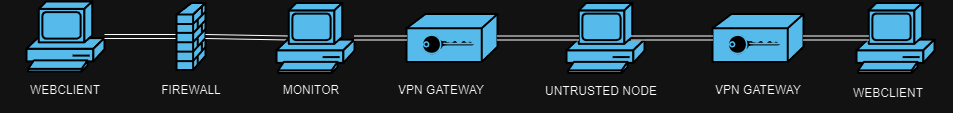
\includegraphics[width=1\textwidth]{SFC.png}  % Sostituisci 'nome_immagine' con il nome del tuo file immagine e l'estensione
    \caption{Esempio di Service Function Chain}
    \label{fig:esempio}
  \end{figure}


Come si può notare, vi sono diversi elementi all'interno di questo esempio.
Per quanto riguarda i vari SF possiamo trovare i seguenti:

\begin{itemize}
    \item \textbf{Firewall}: Si occupa di fare da packet filter fra i due webclient, per filtrare solo i pacchetti che effettivamente sono necessari alla comunicazione
    \item \textbf{Monitor}: Si occupa di monitorare il traffico in transito fra i due nodi, può essere un nodo da interrogare in caso di problematiche all'interno della rete per controllare che il firewall svolga il suo ruolo correttamente.
    \item \textbf{VPN Gateway}: Si occupa di criptare e decriptare il traffico. In questa topologia è fondamentale la loro presenza in quanto vi è un nodo considerato non affidabile, di conseguenza tutte le comunicazioni che passano attraverso quel nodo sono criptografate.
\end{itemize}

L'unione dei tre SF in questo specifico ordine definice una Service Function Chain. E' importante notare che se l'ordine fosse stato diverso (ad esempio mettendo prima i 2 VPN Gateway e dopo il firewall)
la SFC risultante sarebbe stata diversa da quella di partenza, garantendo una ramificazione.

\section{Verefoo}
\subsection{Introduzione}
 Il potenziamento progressivo delle tecnologie appena descritte ha portato rapidamente allo sviluppo di reti  che automatizzavano i lavori di configurazione che solitamente venivano svolti manualmente.
 Un esempio di queste nuove tecnologie viene svolto da VEREFOO\cite{Bringhenti2019}(VErified REfinement and Optimized Orchestration), un framework che si pone diversi obiettivi fra i quali la definizione
ad alto livello dei requisiti di sicurezza di rete, l'allocazione automatica ed ottimale delle varie Service Function per ottenere la maggior efficenza di rete allocando le minori risorse possibili, e la
configurazione automatica delle varie \textit{Network Security Functions}, eliminando l'errore  umano che in reti di grandi dimensioni è solito capitare.
Come è possibile intuire, la sfida di produrre una rete configurata automaticamente e correttamente è molto difficile da ottenere, perciò per assicurare la correttezza formale dei risultati ottenuti da Verefoo
l'intero framework utilizza un metodo formale che si basa sulla risoluzione di un \textit{Maximum Satisfiability Modulo Theories} (MaxSMT) tramite l'engine Z3 di Microsoft.\\
Questo, essendo basato su 3 pilastri quali \textit{Ottimizzazione, Ottimalità e Correttezza Formale}, Verefoo si pone 2 obiettivi da soddisfare:

\begin{enumerate}
    \item L'allocazione ottimale dei vari NSFs
    \item La configurazione ottimale dei vari NSFs.
\end{enumerate}

\subsection{Descrizione del modello}
Il modello di Verefoo, descritto in figura 2.2 richiede in input due elementi fondamentali:

\begin{itemize}
    \item \textbf{Service Graph}: Una topologia logica delle funzioni della rete che insieme formano un collegamento end-to-end. A differenza delle SFC il Service Graph può avere diversi percorsi per collegare due punti nella rete
    presentando la ramificazione tipica della concatenazione di SFC. Durante la creazione del Service Graph non è necessario specificare nessun requisito di sicurezza, come ad esempio Firewall, Monitors o Filtering Databases. 
    \item \textbf{Network Security Requirements}: Sono i requisiti di sicurezza che la rete in output dovrà avere dopo la computazione di Verefoo. Questo elemento è fondamentale per costruire il modello di MaxSMT da risolvere tramite Z3.
    Allo stato attuale, Verefoo consente di avere 3 requisiti di sicurezza principali:
        \begin{enumerate}
            \item \textbf{Reachability Property}: Indica che un nodo Y di destinazione deve essere raggiungibile da un nodo di partenza X in almeno un percoso della topologia.
            \item \textbf{Isolation Property}: Indica che un nodo Y di destinazione \textbf{NON} deve essere raggiungibile da un nodo di partenza X in tutti i possibili percorsi all'interno della topologia.
            \item \textbf{Protection Property}: Indica che la comunicazone tra un nodo di partenza X ed un nodo di destinazione Y deve essere sicura. In questo requisito è anche possibile specificare
                un nodo definito \textit{"Untrusted Node"} ovvero un nodo che potrebbe essere un possibile punto di debolezza nella rete e che quindi deve poter vedere solo il traffico criptografato.
        \end{enumerate}
\end{itemize}


\begin{figure}[h]  % 'h' significa che la figura viene posizionata qui
    \centering
    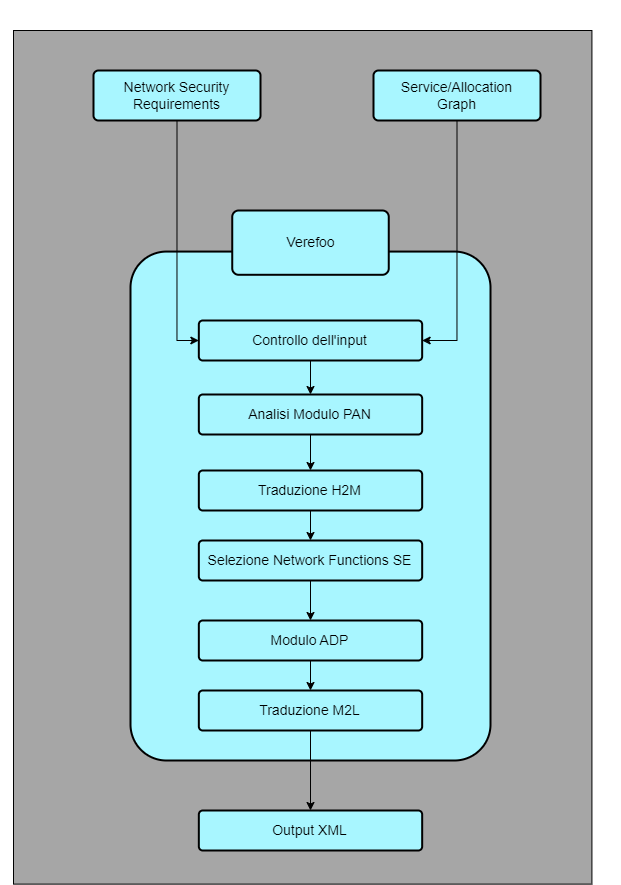
\includegraphics[width=1\textwidth]{VerefooArchitecture.png}  % Sostituisci 'nome_immagine' con il nome del tuo file immagine e l'estensione
    \caption{Architettura di VEREFOO \cite{Bringhenti2019}}
    \label{fig:architettura_verefoo}
  \end{figure}

Successivamente all'input, il framework esegue una serie di passi che possono essere così riassunti:

\begin{enumerate}
    \item \textbf{Fase di controllo dell'input}: In questa fase Verefoo accetta l'input passato sotto forma di file XML e controlla la coerenza dell'input fornito. Il framework 
         oltre ad accettare l'input composto da Service Graph e NSRs accetta anche la possibilità di fornire un \textit{Allocation Graph} al posto del Service Graph(figura 2.3). La
         differenza fondamentale fra i due è che nel secondo oltre ai vari nodi della rete descritti nel Service Graph si specificano anche dei nodi aggiuntivi, chiamati \textit{Allocation Places}
         che rappresentano i punti nella topologia dove è possibile istanziare una funzione di sicurezza di rete.
    \item \textbf{Fase di analisi del modulo PAN}: qui Verefoo esegue un'analisi delle policy che sono state passate in input. Più specificatamente viene controllato che i vari NSRs siano coerenti fra
    loro, evidenziando eventuali errori (ad esempio non si può avere una Reachability Property ed una Isolation Property con gli stessi nodi di partenza e destinazione). Alla fine dell'analisi delle policy
    viene prodotto il numero minimo di vincoli che devono essere rispettati affinchè la topologia soddisfi i NSRs richiesti. In caso di errore un report viene solitamente fornito in output per comprendere 
    il perchè un determinato input non è soddisfabile.
    \item \textbf{Trasformazione a Medium Level Language}: Una volta definiti ad alto livello i vincoli da far rispettare alla topologia, questi vengono tradotti da un linguaggio di alto livello
    ad uno di medio livello tramite il componente H2M. 
    \item  \textbf{Selezione delle Network Function}:Ricevuto l'output dal modulo H2M il modulo Network Functions Selection (SE) si occupa di selezionare da un catalogo le NSF necessarie a rispettare i requisiti
    di alto e medio livello. Questo catalogo è anche accessibile al designer della rete nella fase di design disponibile nella Service GUI di Verefoo.
    \item \textbf{Allocazione, Distribuzione e Piazzamento}:Durante questo passo del framework viene eseguito, come suggerito dal titolo, l'allocazione delle varie funzioni di rete calcolate tramite
    il modulo NF Selection e i vincoli di medio livello tradotti nell'H2M. Questo compito è affidato al modulo ADP che è il cuore di Verefoo, perchè decide in quali punti della rete e con quali configurazioni
    le varie NFs devono essere allocate. L'ADP produce quindi un nuovo Service Graph nel quale sono allocate anche le funzioni di sicurezza di rete, e produce dei file di configurazione per ciascuna funzione allocata
    nel nuovo Service Graph. Queste configurazioni sono create in un linguaggio di basso livello grazie al modulo M2L presente all'interno dell'ADP.
\end{enumerate}


\begin{figure}[h]  % 'h' significa che la figura viene posizionata qui
    \centering
    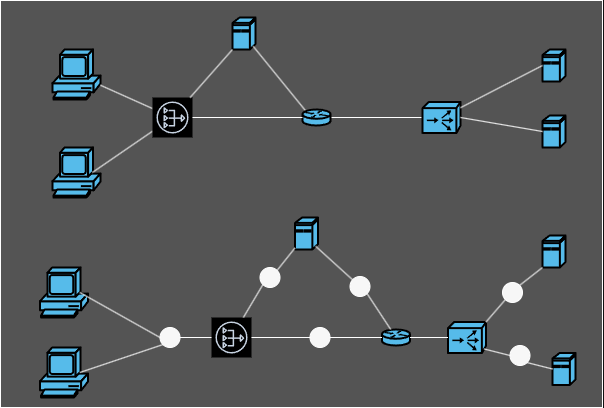
\includegraphics[width=0.9\textwidth]{Service_Allocation_Graph.png}  % Sostituisci 'nome_immagine' con il nome del tuo file immagine e l'estensione
    \caption{Esempi di Service (in alto) e Allocation(in basso) Graphs \cite{Bringhenti2019}}
    \label{fig:AllocationGraph}
  \end{figure}



\section{Definizione ed esempio di Grafo di servizio e di allocazione}

Il primo fondamentale input che deve essere fornito a Verefoo è il grafo di servizio o il grafo di allocazione. 
Viene definito fondamentale perchè è l'unico modo che ha il framework per comprendere la topologia di rete con la quale dovrà interfacciarsi per soddisfare le richieste dell'utente.
Allo stato attuale all'interno di Verefoo è possibile definire come SF le seguenti:

\begin{itemize}
    \item \textbf{Load Balancer}: è uno strumento di controllo di flusso della rete. Il load balancer è infatti in grado di distribuire il carico di lavoro in maniera equa nella rete
        evitando delle situazioni nelle quali alcuni collegamenti fra i nodi risultano sovraccaricati mentre altri inattivi. È quindi in grado di migliorare l'affidabilità e l'efficienza di
        un sistema distribuito.
    \item \textbf{Network Address Translator (NAT)}: è un servizio che consente la traduzione degli indirizzi IP tra due reti. Il suo obiettivo principale è consentire a dispositivi in una rete 
    privata di condividere un singolo indirizzo IP pubblico per accedere a risorse esterne su Internet.  
    \item \textbf{Web Client}: è un'applicazione software o un dispositivo che consente agli utenti di accedere a risorse e servizi su Internet utilizzando il protocollo HTTP (Hypertext Transfer Protocol) o il suo equivalente sicuro HTTPS (Hypertext Transfer Protocol Secure). 
    Questo tipo di client è progettato per interagire con i server web, recuperare informazioni e visualizzare contenuti web.
    \item \textbf{Web Server}: è un software o un'applicazione che fornisce risorse e servizi su Internet, rispondendo alle richieste provenienti dai web client. Il suo ruolo principale è accettare richieste HTTP (Hypertext Transfer Protocol) o HTTPS (Hypertext Transfer Protocol Secure) 
    da parte dei client e inviare loro le risorse richieste.
    \item  \textbf{Packet Filter(Firewall)}: è un componente di sicurezza della rete progettato per monitorare, analizzare e controllare il traffico di rete in base a regole predefinite. La sua funzione principale è quella di decidere quali pacchetti di dati possono attraversare il firewall e raggiungere la destinazione e quali devono essere bloccati.
    \item  \textbf{Web Cache}: è un meccanismo di memorizzazione temporanea che conserva copie di risorse web come pagine HTML, immagini, fogli di stile e altri contenuti multimediali. L'obiettivo principale della web cache è accelerare il caricamento delle pagine web e ridurre il carico sulla rete e sui server web, fornendo ai client risorse già memorizzate localmente anziché scaricarle nuovamente da Internet.
\end{itemize}

Questi elementi possono essere inseriti nella creazione di una rete da fornire a Verefoo. Il framework è in grado di accettare file XML che descrivono il grafo della topologia di rete definendo i nodi nel seguente modo:

\begin{itemize}
    \item \textbf{nome}: é l'indirizzo ip che caratterizza il nodo.
    \item \textbf{funzionalità}: descrive quale delle SF descritte precedentemente il nodo implementa.
    \item \textbf{nodi vicini}: viene fornita una lista di nodi adiacenti al nodo in questione definiti dal loro indirizzo IP. 
    \item  \textbf{configurazione}: viene specificata la configurazione, ove necessaria, per poter istanziare la funzionalità definita al campo precedente.
\end{itemize}


\newpage

\section{Definizione ed esempi delle proprietà di sicurezza}

Le proprietà di sicurezza sono il secondo input che può essere fornito a Verefoo per stabilire i vincoli necessari affinchè
si possa creare una rete sicura. A differenza del primo parametro di input, la definizione della proprietà di sicurezza è 
responsabilità dell'amministratore della rete, in quanto deve decidere tramite le possibilità offerte da Verefoo e dalla GUI ad esso associata
quante e quali proprietà inserire nella propria rete per garantire la sicurezza richiesta.\\
Per garantire flessibilità al framework è possibile inserire le definizioni sia con un linguaggio a basso livello definendo rispetti IP, porte e protocolli
da accettare o rifiutare che con un linguaggio ad alto livello nel quale i vari elementi della rete verranno definiti da dei numeri che poi saranno mappati a degli IP.

I requisiti prodotti all'interno di verefoo saranno formulati con la seguente definizione:

\begin{lstlisting}[caption={Definizione di una proprietà di sicurezza generica},float={h} , label=lst:securityRule]
    [ruleType, IPSrc, IPDst, portSrc, portDst, transportProto]
\end{lstlisting}

\begin{itemize}
    \item \textbf{ruleType}: specifica quale proprietà stiamo definendo. Allo stato attuale del framework ci sono 3 possibili opzione: Reachability Property, Isolation Property e Protection Property.
    \item \textbf{IPSrc}: indica l'indirizzo IP sorgente, cioè il primo nodo della rete dal quale il requisito deve essere applicato.
    \item \textbf{IPDst}: indica l'indirizzo IP destinazione, ovvero l'ultimo nodo della rete dal quale il requisito deve essere applicato.
    \item \textbf{portSrc}:specifica la porta di rete del nodo sorgente che il protocollo di trasporto utilizzerà per inoltrare i pacchetti di rete. In questa opzione è possibile 
        inserire il valore \textit{"*"} che rappresenterà il range di tutte le porte possibili.
    \item \textbf{portDst}:specifica la porta di rete del nodo destinazione che il protocollo di trasporto utilizzerà per ricevere i pacchetti di rete. Come per il valore 
        portSrc anche in questo caso è possibile inserire il valore \textit{"*"} per rappresentare tutte le possibili porte di destinazione.
    \item \textbf{transportProto}:è il campo che specifica quale protocollo di trasporto verrà utilizzato per soddisfare la regola. Allo stato attuale Verefoo consente di utilizzare 2 possibili protocolli, UDP e TCP.
\end{itemize}

\newpage

I campi IPSrc e IPDst non sono limitati a descrivere un singolo host sorgente e un singolo host destinazione per ogni requisito. È infatti possibile utilizzare i due campi per definire anche delle sottoreti. 
Il framework di Verefoo, infatti, definisce gli IP con la classica notazione decimale:

\begin{center}
    \centering  % Aggiunge il comando per centrare il testo
    \textit{ip= ip1.ip2.ip3.ip4}
\end{center}

Ogni elemento da ip1 a ip4 deve appartenere al range [0-255] oppure è possibile utilizzare il valore \textit{"*"} per definire l'intera sottorete.
Grazie a questa implementazione è possibile definire le sottoreti come ad esempio 40.5.0.0\textbackslash16 utilizzando la notazione 40.5.*.* o anche sottoreti
più piccole come 20.1.1.0\textbackslash24 scrivendo 20.1.1.* . \\

Di seguito viene fornita una descrizione più dettagliata dei vari requirements specificabili su Verefoo e di come il framework li traduca in requisiti più generali che la topologia
di rete deve avere affinchè si possa soddisfare la richiesta dell'utente.

\subsection{Reachability Requirements}

I requisiti di raggiungibilità sono definiti nel framework di Verefoo per garantire che un determinato Host sorgente che verrà definito Host-S sia 
in grado di comunicare in maniera diretta e definita con un host destinazione che verrà nominato Host-D. Per garantire ciò è necessario assicurarsi che tutti i 
packet filter presenti nella connessione fra Host-S ed Host-D non scartino mai i pacchetti di questa comunicazione. Per ottenere questo obiettivo è quindi possibile
configurare i packet filter della rete in due modalità: blacklist e whitelist. Nella prima i packet filter faranno transitare tutto il traffico tranne quello specificato
nelle regole definite, mentre nella seconda bloccherà tutto il traffico in entrata escluso quello specificato nelle regole che gli sono state imposte.

Per poter dare per certo che il requisito sia applicabile alla topologia Verefoo svolge le seguenti operazioni:

\begin{enumerate}
    \item  Viene svolto un controllo formale sulla definizione della regola, cioè viene controllata la correttezza di tutti i campi inseriti nella proprietà. In questa prima fase
        Verefoo controlla se gli input inseriti sono tutti presenti e definiti nella maniera corretta (Come ad esempio Stringhe e indirizzi ip come numeri decimali).
    \item Viene svolto un controllo logico sulla definizione della regola, cioè viene controllato che l'indirizzo IP sorgente e quello destinazione appartengano effettivamente a degli host definiti
        nella rete. Inoltre viene controllato anche il protocollo di trasporto, assicurandosi che sia UDP o TCP.
    \item Si ispeziona l'Host-S, e ci si assicura che sia possibile inoltrare il traffico destinato all'Host-D in almeno uno dei nodi adiacenti poichè è sufficiente garantire che esista almeno un percorso
        definito per la comunicazione fra Host-S e Host-D
    \item Infine viene attenzionato l'Host-D, sincerandosi che sia possibile ricevere il traffico proveniente dall'Host-S da almeno uno dei nodi adiacenti, perchè garantisce che almeno un percorso fra l'Host-S
    e l'Host-D sia stato trovato.
\end{enumerate}

Di seguito è possibile trovare un esempio svolto da Verefoo per soddisfare un requisito di raggiungibilità:\\
\begin{figure}[h]  % 'h' significa che la figura viene posizionata qui
    \centering
    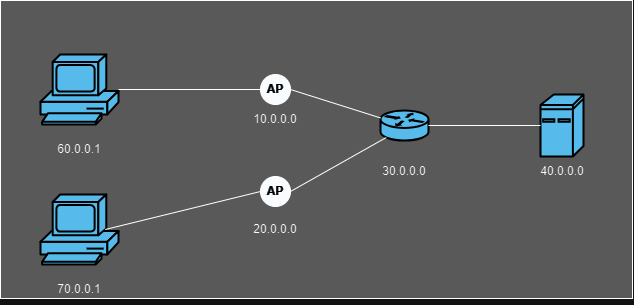
\includegraphics[width=0.8\textwidth]{Reachability.png}  % Sostituisci 'nome_immagine' con il nome del tuo file immagine e l'estensione
    \caption{Grafo di allocazione per requisito di raggiungibilità}
    \label{fig:Reachability}
  \end{figure}

Successivamente è necessario definire la definizione di requisito di raggiungibilità tra l'Host-S 60.0.01 e l'Host-D 40.0.0.0. Nel caso di questo esempio
proveremo a far comunicare i due Host tramite solo il protocollo TCP:
\begin{lstlisting}[style=mystyle,caption={Esempio di requisito di raggiungibilità}]
    <PropertyDefinition>
    <Property graph="0" name="ReachabilityProperty" src="60.0.0.1" dst="40.0.0.0" lv4proto="TCP" src_port="*" dst_port="*"/>
    </PropertyDefinition>
    \end{lstlisting}
    \newpage
Il risultato aspettato è il seguente:\\
\begin{figure}[h]  % 'h' significa che la figura viene posizionata qui
    \centering
    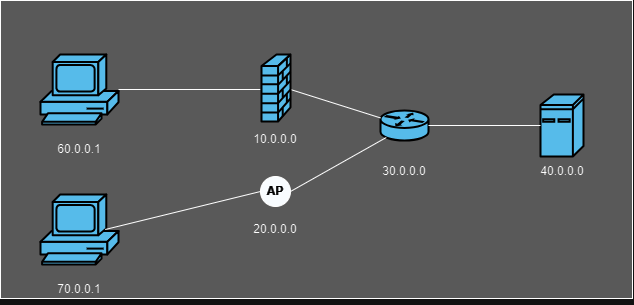
\includegraphics[width=0.8\textwidth]{Reachability_risolta.png}  % Sostituisci 'nome_immagine' con il nome del tuo file immagine e l'estensione
    \caption{Output grafo di esempio per requisito di raggiungibilità}
    \label{fig:Reachability_Soddisfatta}
  \end{figure}


Come si può notare, è stato posto un firewall che funge da packet filter che esclude tutte le comunicazioni uscenti da 60.0.0.1 e dirette a 40.0.0.0 che non utilizzano
il protocollo TCP. Il firewall è quindi stato impostato in blacklist mode negando tutto il traffico che non soddisfa la regola definita sopra.





\subsection{Isolation Requirements}

I requisiti di isolamento sono definiti nel framework di Verefoo per garantire
che un determinato Host sorgente che verrà definito Host-S non sia in grado di comu-
nicare in maniera diretta e definita con un host destinazione che verrà nominato
Host-D. Al fine di poter garantire ciò è necessario che tutti i packet filter presenti nel collegamento tra
Host-S e Host-D scartino a priori ogni pacchetto. In maniera equivalente ai requisiti di raggiungibilità è possibile
implementare nelle reti questo requisito tramite l'utilizzo di packet filter. Analogamente, sarà possibile impostare i
packet filter in blacklist, cioè bloccando solo le comunicazioni che vengono specificate dalle regole di filtraggio, oppure in 
whitelist, permettendo il transito solo dei pacchetti che fanno match con le regole di filtraggio.\\
Affinchè ciò sia implementato correttamente, Verefoo analizza ed opera nel seguente modo ogni requisito di isolamento ricevuto:

\begin{enumerate}
    \item  Come per i requisiti di raggiungibilità, viene svolto un controllo formale sulla definizione della regola, cioè viene controllata la correttezza di tutti i campi inseriti nella proprietà. In questa prima fase
        Verefoo controlla se gli input inseriti sono tutti presenti e definiti nella maniera corretta (Come ad esempio Stringhe e indirizzi ip come numeri decimali).
    \item Viene svolto un controllo logico sulla definizione della regola, cioè viene controllato che l'indirizzo IP sorgente e quello destinazione appartengano effettivamente a degli host definiti
        nella rete. Inoltre viene controllato anche il protocollo di trasporto, assicurandosi che sia UDP o TCP.
    \item Si ispeziona l'Host-S, e ci si assicura che sia possibile inoltrare il traffico destinato all'Host-D in almeno uno dei nodi adiacenti poichè è sufficiente garantire che esista almeno un percorso
        definito per la comunicazione fra Host-S e Host-D
    \item Infine viene attenzionato l'Host-D, sincerandosi che non sia possibile ricevere il traffico proveniente dall'Host-S da nessuno dei nodi adiacenti, così da garantire che non esiste nessun percorso in grado di
    far comunicare l'Host-S e l'Host-D.
\end{enumerate}

Al fine di poter portare all'attenzione un esempio di questo requisito di sicurezza, si utilizzerà la stessa topologia di rete 
consultabile nell'immagine \ref{fig:Reachability}.\\
A differenza del requisito di raggiungibilità, in questo caso la definizione sarà la seguente:\\

\begin{lstlisting}[style=mystyle,caption={Esempio di requisito di isolamento}]
    <PropertyDefinition>
    <Property graph="0" name="IsolationProperty" src="70.0.0.1" dst="40.0.0.0" lv4proto="UDP" />    </PropertyDefinition>
    \end{lstlisting}

In questo caso viene espresso che tutto il traffico proveniente dall'Host-S 70.0.0.1 e diretto all'Host-D 40.0.0.0 che transita
tramite il protocollo di livello 4 UDP, deve essere bloccato e quindi non arrivare a destinazione.
La computazione svolta da Verefoo porta alla seguente:

\begin{figure}[h]  % 'h' significa che la figura viene posizionata qui
    \centering
    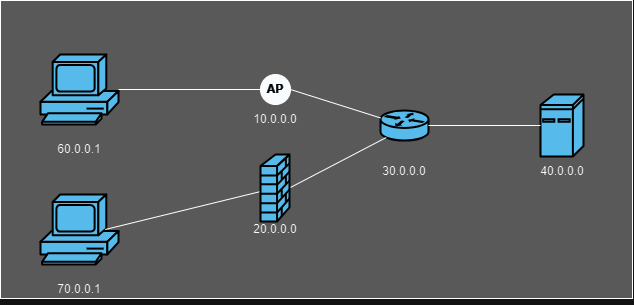
\includegraphics[width=0.8\textwidth]{Isolation_Soddisfatta.png}  % Sostituisci 'nome_immagine' con il nome del tuo file immagine e l'estensione
    \caption{Output grafo di esempio per requisito di isolamento}
    \label{fig:Isolation_Soddisfatta}
  \end{figure}

  A differenza della \ref{fig:Reachability_Soddisfatta}, il packet filter allocato da Verefoo è stato impostato in blacklist
  mode. Facendo ciò le comunicazioni fra i due host 70.0.0.1 e 60.0.0.1 sono ancora garantite e l'unica regola che blocca il traffico
  dati è specifica per le comunicazioni in UDP da 70.0.0.1 a 40.0.0.0.
  \newpage


  \subsection{Protection Requirements}
  I requisiti di protezione sono definiti nel framework di Verefoo per garantire che un determinato Host sorgente che verrà definito Host-S possa 
  comunicare con un host destinazione definito Host-D in maniera sicura garantendo le proprietà di integrità, confidenzialità e segretezza.
  Per assicurare tali prestazioni Verefoo istanzia dei tunnel VPN che vengono allocati nella rete attraverso dei  VPN Gateway in grado di prendere il traffico in ingresso
  del tunnel, criptarlo, farlo transitare all'interno del tunnel e decriptarlo quando il messaggio è arrivato a destinazione. Per fare ciò su Verefoo è presente un translator
  in grado di creare delle configurazioni StrongSwan \cite{strongswan}, un software open-source che permette di istanziare tunnel VPN utilizzando IPsec \cite{ipsec}.\\

  A differenza dei requisiti di raggiungibilità e di isolamento, la definizione della regola varia leggermente aggiungendo qualche campo:

  \begin{lstlisting}[caption={Definizione di una proprietà di protezione},float={h}]
    [ruleType, IPSrc, IPDst, portSrc, portDst, secTecnology,authAlg, encAlg, untrustedNodes, inspectorNodes, untrustedLinks ]
\end{lstlisting}

Come si può notare paragonando questa nuova definizione di regola alla \ref{lst:securityRule} i campi ruleType, IPSrc, IPDst, portSrc e portDst sono gli stessi. Ad essi si aggiungono:

\begin{itemize}
    \item \textbf{secTecnology}: specifica quale tecnologia VPN stiamo definendo.
    \item \textbf{authAlg}: definisce l'algoritmo di autenticazione da utilizzare all'interno del tunnel VPN. 
    \item \textbf{encAlg}: definisce l'algoritmo da utilizzare per eseguire la cifratura dei pacchetti in transito nel tunnel.
    \item \textbf{untrustedNodes}: definisce il set di nodi non sicuri della rete. Questa definizione è fondamentale perchè Verefoo deve conoscere l'insieme dei nodi nel quale è obbligatorio imporre le regole di sicurezza definite dall'utente.
        Solitamente il set di nodi non sicuri è definito dal percorso di collegamento fra l'Host-S e l'host-D, tuttavia è possibile anche aggiungere altri nodi non appartententi al percorso se lo si ritiene necessario.
    \item \textbf{inspectorNodes}: definisce il set di nodi nei quali il traffico deve transitare senza alcuna protezione. Questo set di nodi ha il compito di analizzare il traffico per controllarne la correttezza e la sicurezza, e non potrebbe operare
        se il traffico fosse cifrato. Verefoo ha quindi l'obbligo di trovare una soluzione ottima che permetta ai nodi d'ispezione di analizzare il trafico. 
    \item \textbf{untrustedLinks}: è il set di collegamenti nei quali l'applicazione dei requisiti di sicurezza è obbligatoria.  Similmente al set dei nodi non sicuri, questo parametro è una vera e propria estensione, in quanto tiene in considerazione
        tutti i possibili path che si potrebbero delineare dall'Host-S all'Host-D come link non sicuri. In aggiunta, come accade per gli untrustedNodes, è possibile definire dei link aggiuntivi se lo si ritiene necessario.
\end{itemize}


Al fine di implementare correttamente ogni requisito descritto dalla regola, Verefoo analizza ed opera nel seguente modo ogni requisito di protezione ricevuto:

\begin{enumerate}
    \item  Similmente ai requisiti precedentemente spiegati, viene svolto un controllo formale sulla definizione della regola, cioè viene controllata la correttezza di tutti i campi inseriti nella proprietà. In questa prima fase
        Verefoo controlla se gli input inseriti sono corretti. A differenza dei precedenti requisiti non tutti i parametri nella definizione della regola sono obbligatori, è infatti possibile non definire alcun untrustedNode, inspectorNode o untrustedLink, 
        utilizzando i requisiti di default che il framework calcola.
    \item Viene svolto un controllo logico sulla definizione della regola, cioè viene controllato che l'indirizzo IP sorgente e quello destinazione appartengano effettivamente a degli host definiti
        nella rete.
    \item Si pone attenzione a tutti i possibili flusso di traffico del requisito specificato. Per qualsiasi flusso, ogni qual volta viene incontrato un nodo considerato non sicuro si calcola il numero di nodi precedenti e ci si assicura
        che i nodi che  definiscono e implementano un qualsiasi tipo di protezione siano  sempre in numero maggiore di quelli che invece la rimuovono. Questa condizione è fondamentale per garantire che il traffico che passa attraverso i nodi non sicuri sia 
        sempre cifrato e non ispezionabile dal nodo.
    \item Sempre considerando tutti i possibili flussi di traffico, ogni qual volta viene incontrato un nodo considerato d'ispezione si calcola il numero di nodi precedenti e ci si assicura che i nodi che definiscono  e implementano una qualsiasi protezione siano in numero uguale di quelli che invece la rimuovono.
        Questa condizione è fondamentale per garantire che il traffico che passa attraverso i nodi d'ispezione sia sempre decifrato ed in chiaro, così da essere analizzato.
    \item Infine, come per i due precedenti casi, considerando tutti i flussi di traffico, se si ha un collegamento non sicuro si calcola il numero di nodi precedenti e ci si assicura che i nodi che definiscano e imnplementano una qualsiasi protezione
        siano in numero maggiore di quelli che invece la rimuovono. Sincerandosi di ciò, è possibile garantire che per ogni collegamento non sicuro nel quale il traffico transita, i pacchetti saranno sempre cifrati e non ispezionabili in alcun punto del collegamento.
\end{enumerate}

\newpage
Per poter porre all'attenzione un esempio semplice di requisito di protezione è necessario considerare una topologia differente da quella analizzata nei due precedenti esempi, che è la seguente:

\begin{figure}[h]  % 'h' significa che la figura viene posizionata qui
    \centering
    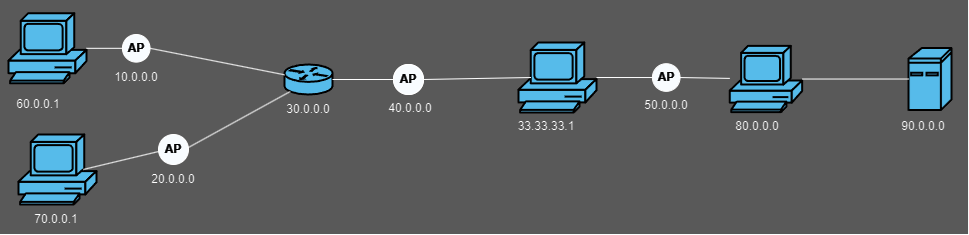
\includegraphics[width=1\textwidth]{EsempioProtection.png}  % Sostituisci 'nome_immagine' con il nome del tuo file immagine e l'estensione
    \caption{Grafo di allocazione d'esempio per requisiti di protezione}
    \label{fig:EsempioProtection}
\end{figure}

In questo esempio, si vuole creare un canale sicuro per far comunicare l'host-S 60.0.0.1 con l'host-D 90.0.0.0. A scopo illustrativo poniamo l'host 33.33.33.1 come nodo non sicuro(untrustedNode)
e l'host 80.0.0.0 come nodo d'ispezione per controllare il traffico in ingresso verso il nodo 90.0.0.0 come se fosse un IDS (inspectorNodes).
Per attuare ciò la definizione da passare in input a Verefoo è la seguente: 

\begin{lstlisting}[style=mystyle,caption={Esempio di requisito di protezione}]
    <PropertyDefinition>
    <Property graph="0" name="ProtectionProperty" src="60.0.0.1"
    dst="90.0.0.0" src_port= "80" dst_port="80">
    <protectionInfo encryptionAlgorithm="AES_128_CBC"
    authenticationAlgorithm="SHA2_256">
    <untrustedNode node="33.33.33.1"/>
    <inspectorNode node= "80.0.0.0"/>
    <securityTechnology>TLS</securityTechnology>
    <securityTechnology>IPSEC</securityTechnology>
    </protectionInfo>
    </Property>
    </PropertyDefinition>
\end{lstlisting}

Una soluzione possibile scelta da Verefoo è la seguente:

\begin{figure}[h]  % 'h' significa che la figura viene posizionata qui
    \centering
    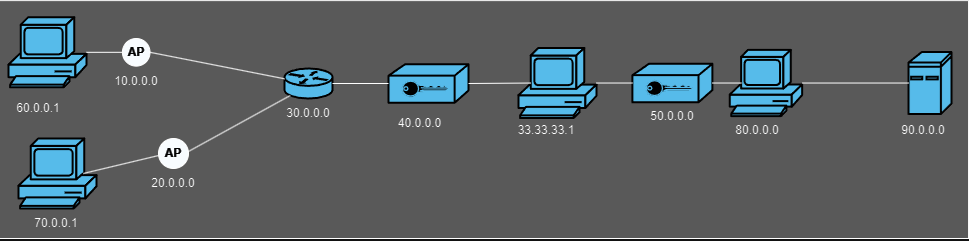
\includegraphics[width=1\textwidth]{ProectionProp.png}  % Sostituisci 'nome_immagine' con il nome del tuo file immagine e l'estensione
    \caption{Output grafo di esempio per requisito di protezione}
    \label{fig:ProtectionRisolta}
\end{figure}

Come si può notare 2 VPN Gateway sono state allocati al fine di garantire i requisiti specificati: il primo al nodo 40.0.0.0
è stato configurato in \textit{"ACCESS MODE"} permettendo a tutti i pacchetti provenienti da 60.0.0.1 e diretti a 90.0.0.0 di entrare nel tunnel VPN, il
secondo invece è stato configurato in \textit{EXIT MODE} così da poter rimuovere la protezione per tutti i pacchetti inserita precedentemente. È inoltre fondamentale
sottolineare come i requisiti che abbiamo richiesto sono stati tutti rispettati. È infatti possibile notare come il nodo considerato non sicuro (33.33.33.1) si trova all'interno del tunnel e ogni
pacchetto che riceve sarà stato precedentemente protetto dal nodo 40.0.0.0. Similmente, il nodo 80.0.0.0 che dovrebbe agire da IDS per la topologia di esempio può svolgere la sua funzione in quanto
tutti i pacchetti in transito vengono precedentemente decifrati dal nodo 50.0.0.0. Infine non avendo specificato alcun collegamento non sicuro verefoo ha garantito soltanto che il collegamento di default
sia sicuro.


\chapter{Docker} \label{ch:docker}

\section{Introduzione a Docker} 

Parte di docker.

\section{Docker Compose}

Parte di Docker compose.

description \cite{noms2020}
\chapter{Obiettivi della tesi} \label{ch:ThesisObj}

Questo capitolo introduce gli obiettivi di questa tesi, descrivendo studi e metodologie utilizzate al fine di raggiungerli.\\
Nei capitoli precedenti è stato infatti descritto lo stato dell'arte di Docker e Verefoo, che sono i due strumenti principali utilizzati per
svolgere questo lavoro di tesi. Il primo è infatti uno strumento fondamentale per poter garantire un ambiente di testing efficiente e isolato, il secondo
invece è il framework principale nel quale la quasi totalità del lavoro si è svolta. Comprendere l'utilizzo correto dei due elementi è quindi di fondamentale importanza al fine di 
poter capire, continuare e migliorare lo stato attuale di Verefoo. Inoltre, molti dei risultati prodotti precedentemente su Verefoo rispetto a questo lavoro pur essendo corretti non
offrivano alcun modo di mostrare in maniera diretta le innovazioni prodotte ai nuovi utenti che si approcciavano al framework. Parte del lavoro svolto è quindi basato sull'ideare e produrre
dei metodi efficaci e semplici per mostrare all'utente le capacità e caratteristiche di Verefoo.\\
Entrando più nello specifico, gli obiettivi della tesi possono essere definiti dal seguente elenco:


\begin{enumerate}
    \item Come primo obiettivo ci si è focalizzati su una demo già presente all'interno dell'ecosistema. All'interno di questa, tuttavia, diversi elementi all'interno erano considerabili obsoleti
        o scorretti, di conseguenza ci si è posti come scopo principale di questa prima parte correggere e perfezionare la demo per mostrare correttamente le potenzialità del framework.
        Allo stato iniziale, il framework era in grado di accettare solo un determinato requisito di sicurezza di rete ovvero
        la \textit{Protection Property} cioè la possibilità di far passare il traffico crittografato da un nodo ad un altro della topologia
        in maniera sicura. Al fine di garantire ciò vengono allocati nella topologia dei VPN Gateway in grado di poter cifrare il traffico in ingresso e decifrare quello in uscita.
        La topologia proposta utilizzerà uno scenario verosimile a quello che ci si potrebbe aspettare in un'azienda di piccole-medie dimensioni, nella quale al fine di poter garantire
        la correttezza dei requisiti proposti, verranno istanziati 6 VPN Gateway. I lavori svolti per questo obiettivo sono consultabili nel capitolo 5 di questa tesi.\newpage
    \item Una volta terminato il restauro della demo sulle VPN, è emersa la necessità di integrare alle funzionalità già presenti la possibilità di configurare anche i packet filter. Come secondo obiettivo ci si è quindi concentrati per trovare una soluzione al fine di poter integrare le varie versioni di Verefoo. 
        Inizialmente il framework era diviso in differenti branch, due dei quali permettevano rispettivamente l'allocazione solamente dei VPN Gateway o dei Firewall configurati come packet filter per garantire la \textit{Isolation Property} e la \textit{Reachability Property}.
        Il traguardo previsto è quello di creare un ulteriore branch che permettesse la fusione dei due precedentemente descritti. Per ottenere ciò diverse soluzioni sono state esplorate. Inizialmente si è pensato di avere una soluzione mista tramite due versioni del framework attive contemporaneamente che comunicavano fra loro in sequenza,
        per poi passare a soluzioni che permettevano con un solo file jar di svolgere entrambe le funzioni in una sola esecuzione. Anche in questo caso sono stati analizzate entrambe le possibili soluzioni per implementare questo obiettivo, sia istanziando prima i Firewall che i gateway VPN che il viceversa.
        La soluzione finale scelta è stata quella di allocare prima i VPN Gateway e successivamente i Firewall, con delle motivazioni a supporto che verranno estese nel capitolo 6.
    \item Concluso il lavoro sul framework è risultato essenziale trovare un modo per mostrare i risultati ottenuti. L'ultimo obiettivo del lavoro svolto è stato quindi la progettazione, lo sviluppo e l'implementazione di un'altra demo, diversa dalla precedente che mostrasse le nuove potenzialità del framework. \\
        A differenza della prima, che da questo momento verrà definita come Demo-A, la seconda, che chiameremo Demo-B, propone un esempio di topologia di rete molto più complessa e con diverse proprietà di sicurezza aggiuntive. Lo sviluppo di questa ha richiesto, come nella precedente, la realizzazione di un'ambiente virtuale dedicato creato con
        Docker-Compose nel quale mostrare come le varie proprità venissero rispettate. Infine, per agevolare i futuri lavori nel framework è stato prodotto in linguaggio Bash un installer per rendere semplice ed immediato l'installazione del framework. Ulteriori approfondimenti sul codice e le scelte effettuate sono descritte nel capitolo 7.
\end{enumerate}

Come ultima appendice al lavoro svolto ai fini di questa tesi, è infine presente una breve conclusione del lavoro che oltre a fare un riassunto generale sugli obiettivi raggiunti definisce i futuri lavori possibili e suggerisce anche alcuni aggiornamenti e perfezionamenti che possono essere svolti nelle demo e nel framework prodotti.

\chapter{Correzione, sviluppo e ottimizzazione Demo A} \label{ch:DemoA}

All'interno di questo capitolo sarà fornita una descrizione completa dei lavori svolti nel primo progetto di demo che è stato preso in analisi inizialmente, corretto e migliorato successivamente.
\\ Inizialmente viene descritta con una breve introduzione gli obiettivi che ci si aspettava di raggiungere con lo sviluppo della demo, i problemi presenti all'inizio del lavoro svolto e le soluzioni possibili attuabili.
\\ Nella seconda parte viene trattato, entrando più nello specifico, l'implementazioni delle soluzioni proposte e presentato il lavoro finale. 
\\ Nell'ultima parte del capitolo viene infine mostrato una prova di correttezza della demo con la verifica dei suoi output e delle sue funzionalità.


\section{Introduzione alla Demo}
Come descritto al Capitolo[\ref{ch:verefoo}] Verefoo è un framework in grado di definire dei requisiti di sicurezza ad alto livello, allocare in maniera ottimale varie Network Security Functions (NSF) all'interno della topologia di rete fornita in input e configurare automaticamente tali funzioni 
automaticamente. Allo stato attuale il framework è ancora in fase di sviluppo e, nonostante si ponga gli obiettivi appena descritti, non tutte le funzionalità sono attualmente possibili all'interno del framework. Più precisamente, varie versioni del framework sono presenti in stato di sviluppo, e ognuna si occupa di allocare una possibile NSF separatamente alle altre.
All'interno di questo capitolo verrà presa in considerazione per il lavoro una di queste possibili versioni, ovvero quella che si occupa della verifica dei Network Security Requirements di protezione, dell'allocazione del numero minimo ottimale di VPN Gateway per rispettare i requisiti in input, e della configurazione di questi ultimi.\\
L'obiettivo principale di questo lavoro di demo è quindi mostrare all'utente come questa versione sia in grado, data una topologia di rete simile a quelle di una azienda di medie dimensioni, di verificare i requisiti, allocare le VPN e configurarle correttamente.
\newpage
Un altro elemento emerso durante i lavori sullo sviluppo di questa demo è stata la difficile accessibilità di quest'ultima. Per far funzionare sia il framework che la demo sono infatti necessari numerosi tool da installare all'interno della macchina in alcune versioni specifiche e potrebbe essere non immediato installare correttamente il dispositivo per far funzionare 
framework e demo. Di conseguenza come obiettivo secondario, ma di uguale importanza è stato prodotto un installer che permette all'utente di ottenere automaticamente tutti i programmi nelle versioni corrette per poter utilizzare il framework a proprio piacimento.
\\
Per portare a termine questi due obiettivi ci si è quindi interfacciati con un progetto di demo che risultava incompleto e mal funzionante. Analizzando più approfonditamente possiamo dividere le modifiche effettuate all'interno di questa demo nei seguenti punti:

\begin{enumerate}
    \item \textbf{Versione Framework}: Il file del framework iniziale era malfunzionante, in quanto ogni qual volta che si provava ad avviarlo il terminale segnalava il file come corrotto ed inutilizzabile.
    \item \textbf{Chiamate API}: La demo utilizzava delle chiamate API considerabili obsolete, di conseguenza qualsiasi relazione con il framework non produceva alcun risultato.
    \item \textbf{Installer}: Come accennato precedentemente la mancanza di un installer della Demo rendeva il framework poco accessibile e di difficile installazione manuale.
    \item \textbf{Certificati VPN}: Alcuni dei certificati di chiavi pubbliche e private erano ormai scaduti, sono quindi stati sostituiti ed i file di configurazione modificati opportunatamente.
    \item \textbf{Docker Compose}: Il file di configurazione dell'ambiente virtuale di Docker Compose conteneva errori e molti dei container non venivano istanziati correttamente.
    \item \textbf{Forwarding Rules}: Alcune forwarding rules all'interno dell'ambiente virtuale erano scorrette, sono state quindi corrette ed aggiornate per garantire la comunicazione fra tutti i nodi della rete.
\end{enumerate}

    
\section{Implementazione}
Welcome to the demo of Verefoo for VPNs. What you will see written here will be a simple stand-alone demo in which the features and capabilities of Verefoo are highlighted.
Before we begin we need to define a network topology that Verefoo will need to relate to, more precisely you will also need to define the respective IP addresses and links between the different nodes.  During the course of the demo, a virtual environment developed with Docker Containers will be instantiated that will reproduce the topology presented in this document.

\begin{figure}[h]  % 'h' significa che la figura viene posizionata qui
    \centering
    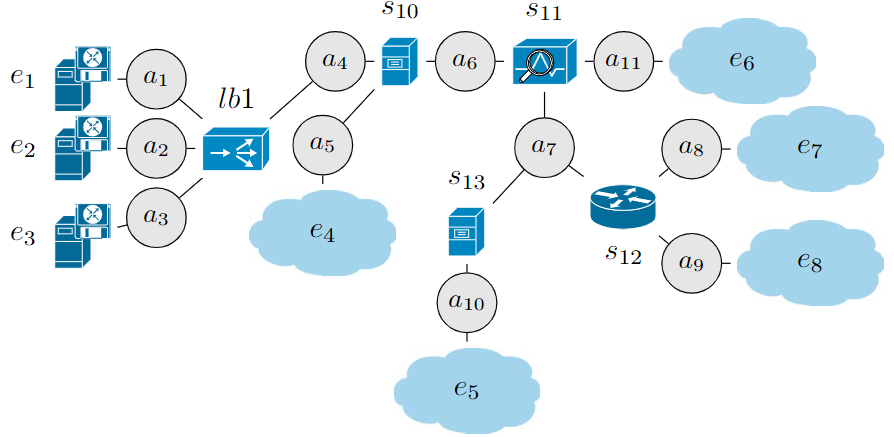
\includegraphics[width=1\textwidth]{VPN_AG.PNG} 
    \caption{Service Graph}
    \label{fig:ServiceGraph}
\end{figure}
As can be seen, the proposed topology has 3 webservers on the left whose traffic is handled by a load balancer and 5 endpoints that are represented by web clients. Within the network there are nodes that will act as monitors, such as node s11, and others that will instead perform the simple forwarder function with their respective static routes. Finally, there are several currently empty nodes that we will call allocation places. Within these nodes, the framework will be able to place network security functions to make sure that the security requirements are working properly within the network. A table is provided below with the definition of each node, its IP address that will be used in the virtual environment, and its functionality within the topology.

\begin{table}[h]
    \centering
    \begin{tabular}{ccc}
        \hline
         Name & IP & Functionality \\
        \hline
        e1 & 130.10.0.1 & Web servers behind load balancer b1 \\
        e2 & 130.10.0.2 & * \\
        e3 & 130.10.0.* & * \\
        e4 & 40.40.41.* & Web Client \\ 
        e5 & 40.40.41.* & Web Client \\
        e6 & 88.80.84.* & Web Client \\
        e7 & 192.168.1.* & Web Client \\
        e8 & 192.168.2.* & Web Client \\
        lb1 & 130.10.0.4 & Load Balancer \\
        s10 & 33.33.33.2 & Web Cache \\
        s11 & 33.33.33.3 & Forwarder \\
        s12 & 220.124.30.1 & Forwarder \\
        s13 & 33.33.33.4 & Forwarder \\
        a7 & 1.0.0.7 & Forwarder \\
        \hline
    \end{tabular}
    \caption{Node definitions and functionalities}
    \label{tab:tabella}
\end{table}


The second and final input that must be provided to the framework is the set of security requirements that the network must have. With this demo, the goal was to have an output topology that contained a large number of VPN Gateways (6), in order to be able to show an example that would come as close as possible to a hypothetical real case of a small-to-medium sized company. In order to be able to achieve a similar topology, the following rules were defined:
\\
\\

\begin{table}[h]
    \centering
    \small
    \begin{tabular}{ccccccccc}
        \hline
         Policy & IPSrc & IPDst & pSrc & pDst & tProto & Confidentiality & Intregrity & Untrusted nodes\\
        \hline
        Protection & 40.40.41.1 & 130.10.0.1 & * & 22 & ANY & AES-256-CBC & SHA2-256 & 33.33.33.2 \\
        Protection & 88.80.84.1 & 130.10.0.* & * & 80 & ANY & AES-256-CBC & SHA2-256 & 33.33.33.2/33.33.33.3 \\
        Protection & 192.168.1.1 & 130.10.0.1 & * & * & ANY & AES-256-CBC & SHA2-256 & 33.33.33.2/33.33.33.3 \\
        Protection & 40.40.42.1 & 192.168.2.1 & * & * & ANY & AES-256-CBC & SHA2-256 & 33.33.33.4/220.124.30.1 \\
        \hline
    \end{tabular}
    \caption{Security Requirements Definition}
    \label{tab:tabella}
\end{table}
\begin{itemize}
    \item \textbf{First Rule}: Web Client e4 must be able to communicate securely with Web Server e1. Traffic originating from e4 can use any port for the transport protocol but the e5 Server must receive data only from port 22. Both UDP and TCP protocols can be used for communications. Finally, node s10 is specified as a non-secure node and through which traffic must pass encrypted.
    \item \textbf{Second Rule}: Web Client e8 must be able to communicate securely with all Web Servers (e1,e2,e3). Traffic originating from e8 can use any port for the transport protocol but the servers must receive data only from port 80. It is possible to use either UDP or TCP protocol for communication. In this case the nodes that are considered non-secure are s10 and s11.
    \item \textbf{Third Rule}: Web Client e7 must be able to communicate securely with Web Server e1. There are no limitations on ports for incoming and outgoing traffic, and any fourth-level protocol can be used. The unsecured nodes, as with the second rule, are s10 and s11. 
    \item \textbf{Fourth Rule}:The Web Client e5 must be able to communicate securely with the Web Client e8. As with the third rule, there are no limitations on the ports and transport protocol to be used. The nodes considered insecure for this rule are s12 and s13.
\end{itemize}

\section{Output}
By providing the previously defined inputs, the framework will look for a solution that not only satisfies all the rules, but also employs the least amount of resources necessary to guarantee these properties. Verefoo will then solve a problem defined as MaxSMT (Maximum Satisfiability Modulo Theories). 
In the specific case of this demo, the result produced in output will be as follows:

\begin{figure}[h]  % 'h' significa che la figura viene posizionata qui
    \centering
    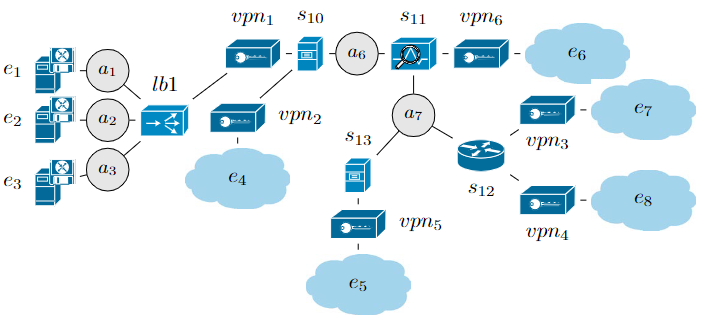
\includegraphics[width=1\textwidth]{VPN_deploy.PNG} 
    \caption{Verefoo Output}
    \label{fig:VPNDeploy}
\end{figure}

As could be imagined, several VPN Gateways were allocated in place of the various Allocation Places defined in the input provided to Verefoo. Given this should be the solution to the problem defined earlier, we will try to test inside the virtual environment the functionality of the various VPN tunnels to make sure that the framework works properly.
Before proceeding, however, it is also important to analyze the various elements that Verefoo has produced. In fact, the framework not only allocates the gateways in the correct places, but also provides an automatic configuration to use. In this specific case, the configuration is as follows:
\\

\begin{table}[ht]
    \centering
    \begin{tabular}{ccccccc}
        \hline
         \# & Action & IPSrc & IPDst & pSrc & pDst & tProto \\
        \hline
        1 & EXIT & 192.168.1.1 & 130.10.0.1 & * & * & ANY \\
        2 & EXIT & 88.80.84.1 & 130.10.0.3 & * & 80 & ANY \\
        3 & EXIT & 40.40.41.1 & 130.10.0.1 & * & 22 & ANY \\
        4 & EXIT & 88.80.84.1 & 130.10.0.1 & * & 80 & ANY \\
        5 & EXIT & 88.80.84.1 & 130.10.0.2 & * & 80 & ANY \\
        6 & ACCESS & 130.10.0.1 & 192.168.1.1 & * & * & ANY \\
        7 & ACCESS & 130.10.0.3 & 88.80.84.1 & 80 & * & ANY \\
        8 & ACCESS & 130.10.0.1 & 40.40.41.1 & 22 & * & ANY \\
        9 & ACCESS & 130.10.0.1 & 88.80.84.1 & 80 & * & ANY \\
        10 & ACCESS & 130.10.0.2 & 88.80.84.1 & 80 & * & ANY\\
        \hline
    \end{tabular}
    \caption{VPN Gateway 1}
    \label{tab:VPN Gateway 1}
\end{table}

\begin{table}[ht]
    \centering
    \begin{tabular}{ccccccc}
        \hline
         \# & Action & IPSrc & IPDst & pSrc & pDst & tProto \\
        \hline
        1 & ACCESS & 40.40.41.1 & 130.10.0.1 & * & 22 & ANY \\
        2 & EXIT & 130.10.0.1 & 40.40.41.1 & 22 & * & ANY \\
        \hline
    \end{tabular}
    \caption{VPN Gateway 2}
    \label{tab:VPN Gateway 2}
\end{table}

\begin{table}[H]
    \centering
    \begin{tabular}{ccccccc}
        \hline
         \# & Action & IPSrc & IPDst & pSrc & pDst & tProto \\
        \hline
        1 & ACCESS & 192.168.1.1 & 130.10.0.1 & * & * & ANY \\
        2 & EXIT & 130.10.0.1 & 192.168.1.1 & * & * & ANY \\
        \hline
    \end{tabular}
    \caption{VPN Gateway 3}
    \label{tab:VPN Gateway 3}
\end{table}

\begin{table}[H]
    \centering
    \begin{tabular}{ccccccc}
        \hline
         \# & Action & IPSrc & IPDst & pSrc & pDst & tProto \\
        \hline
        1 & ACCESS & 192.168.2.1 & 40.40.42.1 & * & * & ANY \\
        2 & EXIT & 40.40.42.1 & 192.168.2.1 & * & * & ANY \\
        \hline
    \end{tabular}
    \caption{VPN Gateway 4}
    \label{tab:VPN Gateway 4}
\end{table}

\begin{table}[H]
    \centering
    \begin{tabular}{ccccccc}
        \hline
         \# & Action & IPSrc & IPDst & pSrc & pDst & tProto \\
        \hline
        1 & ACCESS & 40.40.42.1 & 192.168.2.1 & * & * & ANY \\
        2 & EXIT & 192.168.2.1 & 40.40.42.1 & * & * & ANY \\
        \hline
    \end{tabular}
    \caption{VPN Gateway 5}
    \label{tab:VPN Gateway 5}
\end{table}

\begin{table}[H]
    \centering
    \begin{tabular}{ccccccc}
        \hline
         \# & Action & IPSrc & IPDst & pSrc & pDst & tProto \\
        \hline
        1 & ACCESS & 88.80.84.1 & 130.10.0.1 & * & 80 & ANY \\
        2 & ACCESS & 88.80.84.1 & 130.10.0.2 & * & 80 & ANY \\
        3 & ACCESS & 88.80.84.1 & 130.10.0.3 & * & 80 & ANY \\
        4 & EXIT & 130.10.0.1 & 88.80.84.1 & 80 & * & ANY \\
        5 & EXIT & 130.10.0.2 & 88.80.84.1 & 80 & * & ANY \\
        6 & EXIT & 130.10.0.3 & 88.80.84.1 & 80 & * & ANY \\
        \hline
    \end{tabular}
    \caption{VPN Gateway 6}
    \label{tab:VPN Gateway 6}
\end{table}

\section{Verifiche e Test}
\chapter{Merge} \label{ch:MergeChapter}

Merge works of the 2 verefoo versions
\lstdefinestyle{yaml}{
     basicstyle=\color{red}\footnotesize,
     rulecolor=\color{black},
     string=[s]{'}{'},
     stringstyle=\color{red},
     comment=[l]{:},
     commentstyle=\color{black},
     morecomment=[l]{-}
 }

 \lstdefinestyle{bashstyle}{
    language=bash,
    basicstyle=\small\ttfamily,
    backgroundcolor=\color{gray!10},
    keywordstyle=\color{blue},
    commentstyle=\color{green!50!black},
    stringstyle=\color{red},
    showstringspaces=false,
    morekeywords={mkdir, ls, cd, mv, rm, chmod, sudo}
}

\chapter{Design, progetto e sviluppo Demo B} \label{ch:DemoB}
All'interno di questo capitolo viene descritto il deisgn, lo sviluppo e la realizzazione del secondo lavoro di Demo prodotto.
Questo lavoro si differenzia dal precedente descritto al Capitolo [\ref{ch:DemoA}] in quanto ogni elemento appartenente alla Demo è stato creato da zero,
senza avere nessun riferimento precedente.\\
Inizialmente verrà fornita una breve introduzione alla demo, descrivendo obiettivi e motivazioni che han portato allo sviluppo, successivamente invece verrà
descritta la topologia di rete progettata e i requisiti di sicurezza richiesti, analizzando le motivazioni che hanno portato alla scelta di questi ultimi.\\
Terminata l'introduzione verrà poi descritto lo sviluppo dell'ambiente virtuale, facendo riferimenti a snippet di codici effettivamente implementati all'interno dell'ambiente e 
descrivendo accuratamente i file utilizzati per creare immagini e container all'interno di Docker Compose.\\
Infine l'ultima parte del capitolo, in maniera simile al capitolo sulla Demo A, proporrà dei test e delle verifiche della correttezza degli output forniti da Verefoo.

\section{Introduzione}
Come è stato ampiamente discusso nel Capitolo [\ref{ch:MergeChapter}] la nuova versione di Verefoo prodotta è ora in grado di allocare, in un'unica iterazione, contemporanemante due tipi di Network Security Functions:
i Firewall configurati come dei Packet Filter e dei VPN Gateway che consentono l'autenticazione e la cifratura dei pacchetti durante le comunicazioni fra due endpoint. Tramite queste novità è quindi possibile definire contemporanemante
sia le proprietà di isolamento e raggiungibilità che quelle di protezione, garantendo flessibilità all'utente. Essendo questo un risultato definibile come una milestone nel percorso di sviluppo di Verefoo si è pensato di realizzare una Demo che
possa mostrare i progressi raggiunti tramite l'istanziazione di un nuovo ambiente virtuale. In questo caso rispetto al precedente non ci si è concentrati sul definire dei requisiti il più simile possibile a quelli di una ipotetica azienda di medie dimensioni
quanto più a mostrare in maniera evidente come tutti e 3 i requisiti di sicurezza vengono rispettati. Nonostante questo obiettivo si è però deciso di utilizzare una topologia più complessa rispetto a quella della Demo A, così da mostrare anche come con diversi elementi
che aumentano il carico computazionale del framework, la soluzione che viene fornita in output è computata in maniera rapida, ottimale e sopratutto corretta. \\
Avendo già sviluppato un installer per la Demo A (paragrafo \ref{sec:Installer}) all'interno del repository non è stato necessario crearne uno nuovo, in quanto i package utilizzati in questa Demo sono gli stessi di quella precedente, è quindi stato fornitto all'utente lo stesso 
file.

\section{Implementazione}
Per raggiungere gli obiettivi descritti nell'introduzione si è pensato di creare molti più host rispetto alle versioni precedenti. In questo modo è possibile notare anche le potenzialità di virtualizzazione che l'utilizzo dei container tramite Docker Compose ci permette di avere.
Inoltre ogni host che viene rappresentato in figura non rappresenterà un unico elemento all'interno della topologia ma uno dei possibili host della sottorete definita nel quadrato in cui l'host è contenuto. Di seguito viene quindi fornita una rappresentazione grafica della topologia: 
\begin{figure}[h]  % 'h' significa che la figura viene posizionata qui
    \centering
    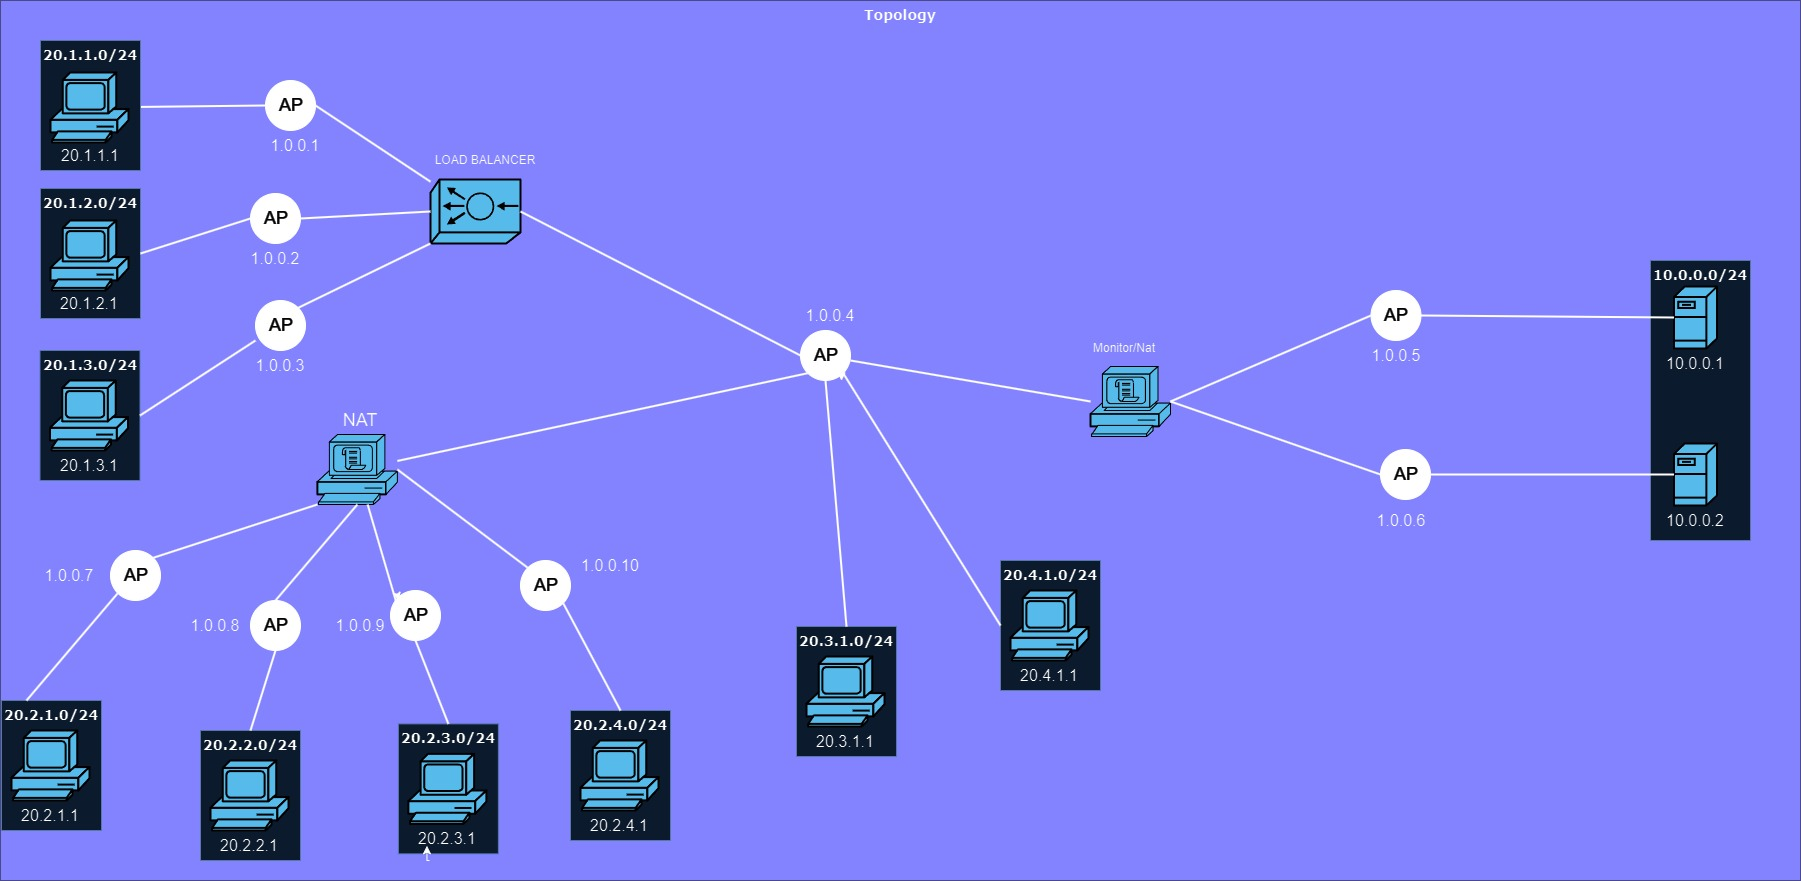
\includegraphics[width=1\textwidth]{Allocation_Graph.jpg} 
    \caption{Grafo di Allocazione della Demo B}
    \label{fig:AllocationGraphB}
\end{figure}

Entrando più nel dettaglio è possibile notare diversi gruppi di host, che rappresentano delle ipotetiche sedi aziendali separate. La prima, in alto a sinistra, viene descritta con la sottorete 20.1.0.0/16. All'interno di questo cluster sono presenti 
tre sottoreti rappresentate dagli ip 20.1.1.0/24, 20.1.2.0/24, 20.1.3.0/24. Le comunicazioni di queste sottoreti vengono regolate da un Load Balancer, che in caso di congestione del traffico decide arbitrariamente in quale nodo della rete inoltrare il traffico
per decongestionare alcuni collegamenti. La seconda sede aziendale è rappresentata in basso a sinistra dalla rete 20.2.0.0/16. Come per la prima sede sono presenti 4 sottoreti di host definite dagli ip 20.2.1.0/24, 20.2.2.0/24, 20.2.3.0/24, 20.2.4.0/24. Diversamente dalla 
prima, all'esterno del cluster 20.2.0.0/16 è presente un NAT che si occupa di mascherare gli indirizzi ip all'interno della rete con il resto della topologia. In basso sono inoltre presenti altre due sedi più piccole delle precedenti, definite dalle sottoreti 20.3.1.0/24 
e 20.4.1.0/24, queste dovrebbero simulare eventuali dipendenti in smart working che quindi non si connettono da una grande rete aziendale ma dalla propria rete di casa privata.\\
Sulla destra è invece presente una Server Farm definita dalla rete 10.0.0.0/24; all'interno sono stati definiti due Web Server con IP 10.0.0.1 e 10.0.0.2.  Infine è presente un nodo che funge da monitor (Mnt) per ispezionare il traffico in entrata ed uscita dai Web Server.
La topologia appena descritta può essere sintetizzata dalla tabella seguente:
\begin{table}
    \centering
    \begin{tabular}{ccc}
        \hline
         Name & IP & Functionality \\
        \hline
        C1-1 & 20.1.1.1 & Web Client behind load balancer \\
        C1-2 & 20.1.2.1 & Web Client behind load balancer \\
        C1-3 & 20.1.3.1 & Web Client behind load balancer \\
        Lb & 33.33.33.1 & Load balancer \\ 
        C2-1 & 20.2.1.1 & Web Client behind NAT \\
        C2-2 & 20.2.2.1 & Web Client behind NAT \\
        C2-3 & 20.2.3.1 & Web Client behind NAT \\
        C2-4 & 20.2.4.1 & Web Client behind NAT \\
        FW1 & 33.33.33.3 & Forwarder \\
        C3-1 & 20.3.1.1 & Web Client \\
        C4-1 & 20.4.1.1 & Web Client \\
        Mnt & 33.33.33.2 & Traffic Monitor \\
        S1 & 10.0.0.1 & Web Server \\
        S2 & 10.0.0.2 & Web Server \\
        \hline
    \end{tabular}
    \caption{Definizione nodi della topologia per Demo B}
    \label{tab:tabella}
\end{table}

Entrambi i server sono i punti d'interesse più importanti della topologia perchè le comunicazioni che verranno effettuate durante la simulazione utilizzeranno come 
uno dei due host almeno uno dei due server. Entrando più nello specifico l'obiettivo dei requisiti di sicurezza di isolamento e raggiungibilità sarà quello di rendere le 
comunicazioni della prima sede possibili solo con il server 10.0.0.2, della seconda sede solo con il server di 10.0.0.1 e delle restanti due sedi con entrambi i server. Per quanto riguarda
invece i requisiti di protezione l'obiettivo che si ci si è prefissati è quello di inserire almeno 2 VPN Gateway affinchè un host specifico all'interno della rete possa comunicare in maniera
sicura con i server per lo scambio di informazioni riservate. Di conseguenza è stato scelto uno degli host della prima sede, immaginandosi quindi la rete 20.1.0.0/16 come la sede centrale dell'azienda.
La definizione dei requisiti di sicurezza è quindi definibile in input al framework tramite la seguente tabella:

\begin{table}[H]
    \centering
    \small
    \setlength{\tabcolsep}{2pt} % Riduci il padding delle colonne
   \begin{tabular}{ccccccccc}
        \hline
         Policy & IPSrc & IPDst & pSrc & pDst & tProto & Confidentiality & Intregrity & Untrusted nodes\\
        \hline
        Isolation & 20.1.1.1 & 10.0.0.1 & * & * & ANY & // & // & // \\
        Reachability & 20.1.1.1 & 10.0.0.2 & * & * & ANY & // & // & // \\
        \hline
        Isolation & 20.1.2.1 & 10.0.0.1 & * & * & ANY & // & // & // \\
        Reachability & 20.1.2.1 & 10.0.0.2 & * & * & ANY & // & // & // \\
        \hline
        Isolation & 20.1.3.1 & 10.0.0.1 & * & * & ANY & // & // & // \\
        Reachability & 20.1.3.1 & 10.0.0.2 & * & * & ANY & // & // & // \\
        \hline
        Reachability & 20.2.1.1 & 10.0.0.1 & * & * & ANY & // & // & // \\
        Isolation & 20.2.1.1 & 10.0.0.2 & * & * & ANY & // & // & // \\
        \hline
        Reachability & 20.2.2.1 & 10.0.0.1 & * & * & ANY & // & // & // \\
        Isolation & 20.2.2.1 & 10.0.0.2 & * & * & ANY & // & // & // \\
        \hline
        Reachability & 20.2.3.1 & 10.0.0.1 & * & * & ANY & // & // & // \\
        Isolation & 20.2.3.1 & 10.0.0.2 & * & * & ANY & // & // & // \\
        \hline
        Reachability & 20.2.4.1 & 10.0.0.1 & * & * & ANY & // & // & // \\
        Isolation & 20.2.4.1 & 10.0.0.2 & * & * & ANY & // & // & // \\
        \hline
        Reachability & 20.3.1.1 & 10.0.0.1 & * & * & ANY & // & // & // \\
        Reachability & 20.3.1.1 & 10.0.0.2 & * & * & ANY & // & // & // \\
        \hline
        Reachability & 20.4.1.1 & 10.0.0.1 & * & * & ANY & // & // & // \\
        Reachability & 20.4.1.1 & 10.0.0.2 & * & * & ANY & // & // & // \\
        \hline
        Protection & 20.1.1.1 & 10.0.0.2 & * & 22 & ANY & AES-256-CBC & SHA2-256 & 33.33.33.2 \\
        \hline
    \end{tabular}
    \caption{Definizione requisiti di sicurezza della topologia per Demo B}
    \label{tab:tabellaNodiB}
\end{table}

\begin{itemize}
    \item \textbf{Prima coppia di Regole}: Il Web Client C1-1 deve poter essere sempre in grado di raggiungere con almeno un percorso il server S2 e non deve poter raggiungere con alcun percorso il server S1 all'interno della topologia. Per entrambe le regole non ci sono limitazioni di utilizzo sulla porta e sul protocollo di quarto livello, è quindi possibile utilizzare una qualsiasi porta nel range [0-65536] sia per il traffico in entrata che in uscita ed un protocollo a scelta fra UDP e TCP.
    \item \textbf{Seconda coppia di Regole}: Il Web Client C1-2 deve poter essere sempre in grado di raggiungere con almeno un percorso il server S2 e non deve poter raggiungere con alcun percorso il server S1 all'interno della topologia. Per entrambe le regole non ci sono limitazioni di utilizzo sulla porta e sul protocollo di quarto livello, è quindi possibile utilizzare una qualsiasi porta nel range [0-65536] sia per il traffico in entrata che in uscita ed un protocollo a scelta fra UDP e TCP. 
    \item \textbf{Terza coppia di Regole}: Il Web Client C1-1 deve poter essere sempre in grado di raggiungere con almeno un percorso il server S2 e non deve poter raggiungere con alcun percorso il server S1 all'interno della topologia. Per entrambe le regole non ci sono limitazioni di utilizzo sulla porta e sul protocollo di quarto livello, è quindi possibile utilizzare una qualsiasi porta nel range [0-65536] sia per il traffico in entrata che in uscita ed un protocollo a scelta fra UDP e TCP.
    \item \textbf{Quarta coppia di Regole}: Il Web Client C2-1 deve poter essere sempre in grado di raggiungere con almeno un percorso il server S1 e non deve poter raggiungere con alcun percorso il server S2 all'interno della topologia. Per entrambe le regole non ci sono limitazioni di utilizzo sulla porta e sul protocollo di quarto livello, è quindi possibile utilizzare una qualsiasi porta nel range [0-65536] sia per il traffico in entrata che in uscita ed un protocollo a scelta fra UDP e TCP.
    \item \textbf{Quinta coppia di Regole}: Il Web Client C2-2 deve poter essere sempre in grado di raggiungere con almeno un percorso il server S1 e non deve poter raggiungere con alcun percorso il server S2 all'interno della topologia. Per entrambe le regole non ci sono limitazioni di utilizzo sulla porta e sul protocollo di quarto livello, è quindi possibile utilizzare una qualsiasi porta nel range [0-65536] sia per il traffico in entrata che in uscita ed un protocollo a scelta fra UDP e TCP.
    \item \textbf{Sesta coppia di Regole}: Il Web Client C2-3 deve poter essere sempre in grado di raggiungere con almeno un percorso il server S1 e non deve poter raggiungere con alcun percorso il server S2 all'interno della topologia. Per entrambe le regole non ci sono limitazioni di utilizzo sulla porta e sul protocollo di quarto livello, è quindi possibile utilizzare una qualsiasi porta nel range [0-65536] sia per il traffico in entrata che in uscita ed un protocollo a scelta fra UDP e TCP.
    \item \textbf{Settima coppia di Regole}: Il Web Client C2-4 deve poter essere sempre in grado di raggiungere con almeno un percorso il server S1 e non deve poter raggiungere con alcun percorso il server S2 all'interno della topologia. Per entrambe le regole non ci sono limitazioni di utilizzo sulla porta e sul protocollo di quarto livello, è quindi possibile utilizzare una qualsiasi porta nel range [0-65536] sia per il traffico in entrata che in uscita ed un protocollo a scelta fra UDP e TCP.
    \item \textbf{Ottava coppia di Regole}: Il Web Client C3-1 deve poter essere sempre in grado di raggiungere con almeno un percorso il server S1 e con almeno un percorso anche il server S2. Per entrambe le regole non ci sono limitazioni di utilizzo sulla porta e sul protocollo di quarto livello, è quindi possibile utilizzare una qualsiasi porta nel range [0-65536] sia per il traffico in entrata che in uscita ed un protocollo a scelta fra UDP e TCP.
    \item \textbf{Nona coppia di Regole}: Il Web Client C4-1 deve poter essere sempre in grado di raggiungere con almeno un percorso il server S1 e con almeno un percorso anche il server S2. Per entrambe le regole non ci sono limitazioni di utilizzo sulla porta e sul protocollo di quarto livello, è quindi possibile utilizzare una qualsiasi porta nel range [0-65536] sia per il traffico in entrata che in uscita ed un protocollo a scelta fra UDP e TCP.
    \item \textbf{Decima Regola}: Il Web Client C1-1 deve poter comunicare in maniera sicura con il Web Server S2. Il traffico originato da C1-1 può utilizzare qualsiasi porta di uscita per il protocollo di trasporto ma il Server S2 deve ricevere i dati in ingresso unicamente dalla porta 22. È possibile utilizzare sia il protocollo UDP che TCP per il trasporto. Viene specificato infine il nodo Mnt come nodo non sicuro e attraverso il quale il traffico deve passare cifrato.
\end{itemize}

Come ampiamente è stato già discusso per la Demo A, anche in questo caso non è sufficiente definire le regole su Verefoo per assicurarsi di avere una soluzione ottimale, ma è necessario creare un ambiente isolato in grado di testare la correttezza delle configurazioni prodotte da Verefoo. Anche in questo caso è stato scelto
di utilizzare Docker Compose per la realizzazione di una rete virtuale, nella quale ogni host, server, forwarder, firewall e VPN gateway è rappresentato univocamente da un container in esecuzione. Di seguito viene presentata una parte dei servizi definiti all'interno del docker-compose file per istanziare una topologia del genere:

\begin{lstlisting}[style=yaml,caption={Definizione di Services dell'ambiente virtuale DemoB},label=composeDemoA]
    server1:
    container_name: server1
    hostname: server1
    image: endpoint
    cap_add:
      - NET_ADMIN
    command: >-
      sh -c "route del default && route add -net 0.0.0.0 netmask 0.0.0.0 gw
      10.0.0.100 && tail -F anything"
    networks:
      servers:
        ipv4_address: 10.0.0.1
  server2:
    container_name: server2
    hostname: server2
    image: endpoint
    cap_add:
      - NET_ADMIN
    command: >-
      sh -c "route del default && route add -net 0.0.0.0 netmask 0.0.0.0 gw
      10.0.0.199 && tail -F anything"
    networks:
      servers:
        ipv4_address: 10.0.0.2

   forwarder1:
     container_name: forwarder1
     hostname: forwarder1
     image: endpoint
     cap_add:
        - NET_ADMIN
     volumes:
        - './RouterVPNConfig:/mnt:ro'
     command: sh -c "/mnt/staticroutes/forone && tail -F anything"
     networks:
        servers:
            ipv4_address: 10.0.0.100
          forwarder1_vpn3:
            ipv4_address: 130.0.3.2
          forwarder1_fw: 
            ipv4_address: 80.0.1.2
   client1_1:
            container_name: client1_1
            hostname: client1_1
            image: endpoint
            cap_add:
              - NET_ADMIN
            command: >-
              sh -c "route del default && route add -net 0.0.0.0 netmask 0.0.0.0 gw
              20.1.1.100 && tail -F anything"
            networks:
              clients1_1:
                ipv4_address: 20.1.1.1
    
\end{lstlisting}


In questo design, diversamente dal precedente, è possibile notare come i due Web Server condividono la stessa rete, ma viene impostato un default gateway differente. Questa scelta è stata necessaria in quanto 
come è possibile notare nella figura (\ref{fig:AllocationGraphB}) sono presenti due diversi allocation place per collegare i due elementi. Grazie a questa configurazione sarà quindi possibile instanziare Network Security Functions
differenti a seconda del server con cui si comunica. Nelle definizioni d'esempio è presente pure quella di un forwarder, in questo caso seppur l'immagine utilizzata per la costruzione del container è identica a quella di un endpoint generico
durante l'instanziazione del container viene eseguito un comando bash aggiuntivo che carica il file "forone" dalle static route. Tramite ciò è possibile definire tutti i forwarding path per ogni elemento che non influenza le proprietà di sicurezza della rete.\\
Per quanto riguarda i Web Client all'interno della topologia la singola definizione è identica a quella proposta all'interno della Demo A con l'unica maggiore differenza è che è stato scelto l'ip terminante con \textit{".100"} come il default gateway per ogni 
host.\\ \\ 
Entrando più nello specifico, è stato necessario definire delle immagini dalle quali istanziare i container grazie al Docker deamon. Per tutte le immagini si è deciso di utilizzare delle immagini di alpine, una distribuzione Linux estremamente leggera in termini di dimensioni su disco e generalmente sicura, nella quale sono poi installabili eventuali
package aggiuntivi che permettono di creare delle versioni custom dell'immagine a seconda di ciò che vogliamo far svolgere al container. Nel caso degli endpoint la definizione del Dockerfile è la seguente:


\begin{lstlisting}[style=bashstyle, caption={Definizione Dockerfile Endpoint}, label=lst:bash-dockerfileEnd,numbers=left]
    FROM alpine:latest

    RUN apk update
    RUN apk add hping3 --update-cache --repository http://dl-cdn.alpinelinux.org/alpine/edge/testing
    RUN apk add tcpdump
    RUN apk add  net-tools 
    ENV PS1='\h:\w\$ '
    
    CMD ["/bin/sh"];
\end{lstlisting}

Partendo dall'ultima immagine disponibile nel repository generale di Docker viene installato un container alpine, successivamente viene fatto un update dei vari package disponibili e installato il package hping3 che consente di inviare dei pacchetti ICMP/UDP/TCP
e tracciare il loro percorso all'interno della rete utilizzando il comando \textit{"--traceroute"}. Questo package è  puramente necessario per eseguire le operazioni di debug e controllo all'interno della rete. Completano il container i package tcpdump e net-tools
che permettono rispettivamente di osservare le interfacce di rete per osservare i pacchetti in transito e di eseguire comandi per la configurazione di rete come ifconfig, arp. ipmaddr eccetera.\\

Nonostante gli output non siano ancora stati prodotti, dai requisiti di sicurezza ci si aspetta di avere degli allocation places nel quale verranno istanziati Firewall e VPN. Di conseguenza dei Dockerfile sono stati scritti per la futura allocazione di queste Security Network Functions.
Di seguito viene fornito il Dockerfile dei container destinati a diventare Firewall:
\begin{lstlisting}[style=bashstyle, caption={Definizione Dockerfile Firewall}, label=lst:bash-dockerfileEnd,numbers=left]
    FROM alpine:latest

    RUN apk update
    RUN apk add iptables sudo
    RUN apk add tcpdump
    RUN apk add bash
    RUN apk add --no-cache quagga \
     && touch /etc/quagga/zebra.conf \
     && touch /etc/quagga/vtysh.conf \
     && touch /etc/quagga/ripd.conf
    ENV PS1='\h:\w\$ '     
    CMD ["/bin/sh"];
\end{lstlisting}
All'interno di questa configurazione di alpine viene installato il package iptables, che è necessario in quanto permette di definire a livello software un firewall, di monitorare il traffico in ingresso ed uscita dal nodo e di scartare 
eventuali pacchetti che non soddisfano la configurazione. A questo package si aggiunge quagga che è un package in grado di definire delle funzioni di routing avanzate per comunicazioni basate su TCP o IP. All'interno della cartella di installazione di quagga vengono
poi definiti dei file di configurazione necessari ad un corretto funzionamento del software. I packages di tcpdump e bash sono presenti solamente per effettuare operazioni di debug e test.\\

Infine è disponibile una definizione dell'immagine di un ipotetico VPN Gateway:
\begin{lstlisting}[style=bashstyle, caption={Definizione Dockerfile VPN Gateway}, label=lst:bash-dockerfileEnd,numbers=left]
    FROM alpine:latest
    RUN apk update
    RUN apk add  net-tools 
    RUN apk add iptables sudo
    RUN apk add tcpdump
    RUN apk add --update strongswan && \
        rm -rf /var/cache/apk/* && \
        mkdir -p /etc/strongswan
    ENV PS1='\h:\w\$ ' 
    CMD ["/bin/sh"]
\end{lstlisting}

Quest'ultima configurazione oltre ad utilizzare alcuni packages come iptables, tcpdump e net-tools discussi precedentemente installa il software fondamentale per effettuare operazioni di tunneling VPN ovvero strongswan. Questo package è in grado di accettare
le configurazioni che vengono fornite in output dal Translator di Verefoo, velocizzando quindi le operazioni di testing delle configurazioni prodotte.

\section{Output}
\subsection{Topologia di Rete}
Una volta definito tutto il necessario affinchè sia possibile istanziare in sicurezza e in maniera corretta un ambiente virtuale basato sui container Docker, è possibile iniziare a verificare la correttezza della nuova versione del framework analizzando i suoi output.
È importante sottolineare che il numero di allocation places definiti in input è volutamente inferiore a quello necessario per rispettare i vincoli in maniera ottimale. Tramite questa scelta di design è quindi possibile controllare che i nuovi allocation places istanziati dopo 
l'allocazione delle VPN vengano considerati nel calcolo delle soluzioni ottimali.\\
Fornendo quindi l'output definito nel paragrafo precedente la soluzione prodotta in output da Verefoo è la seguente:

\begin{figure}[h]  % 'h' significa che la figura viene posizionata qui
    \centering
    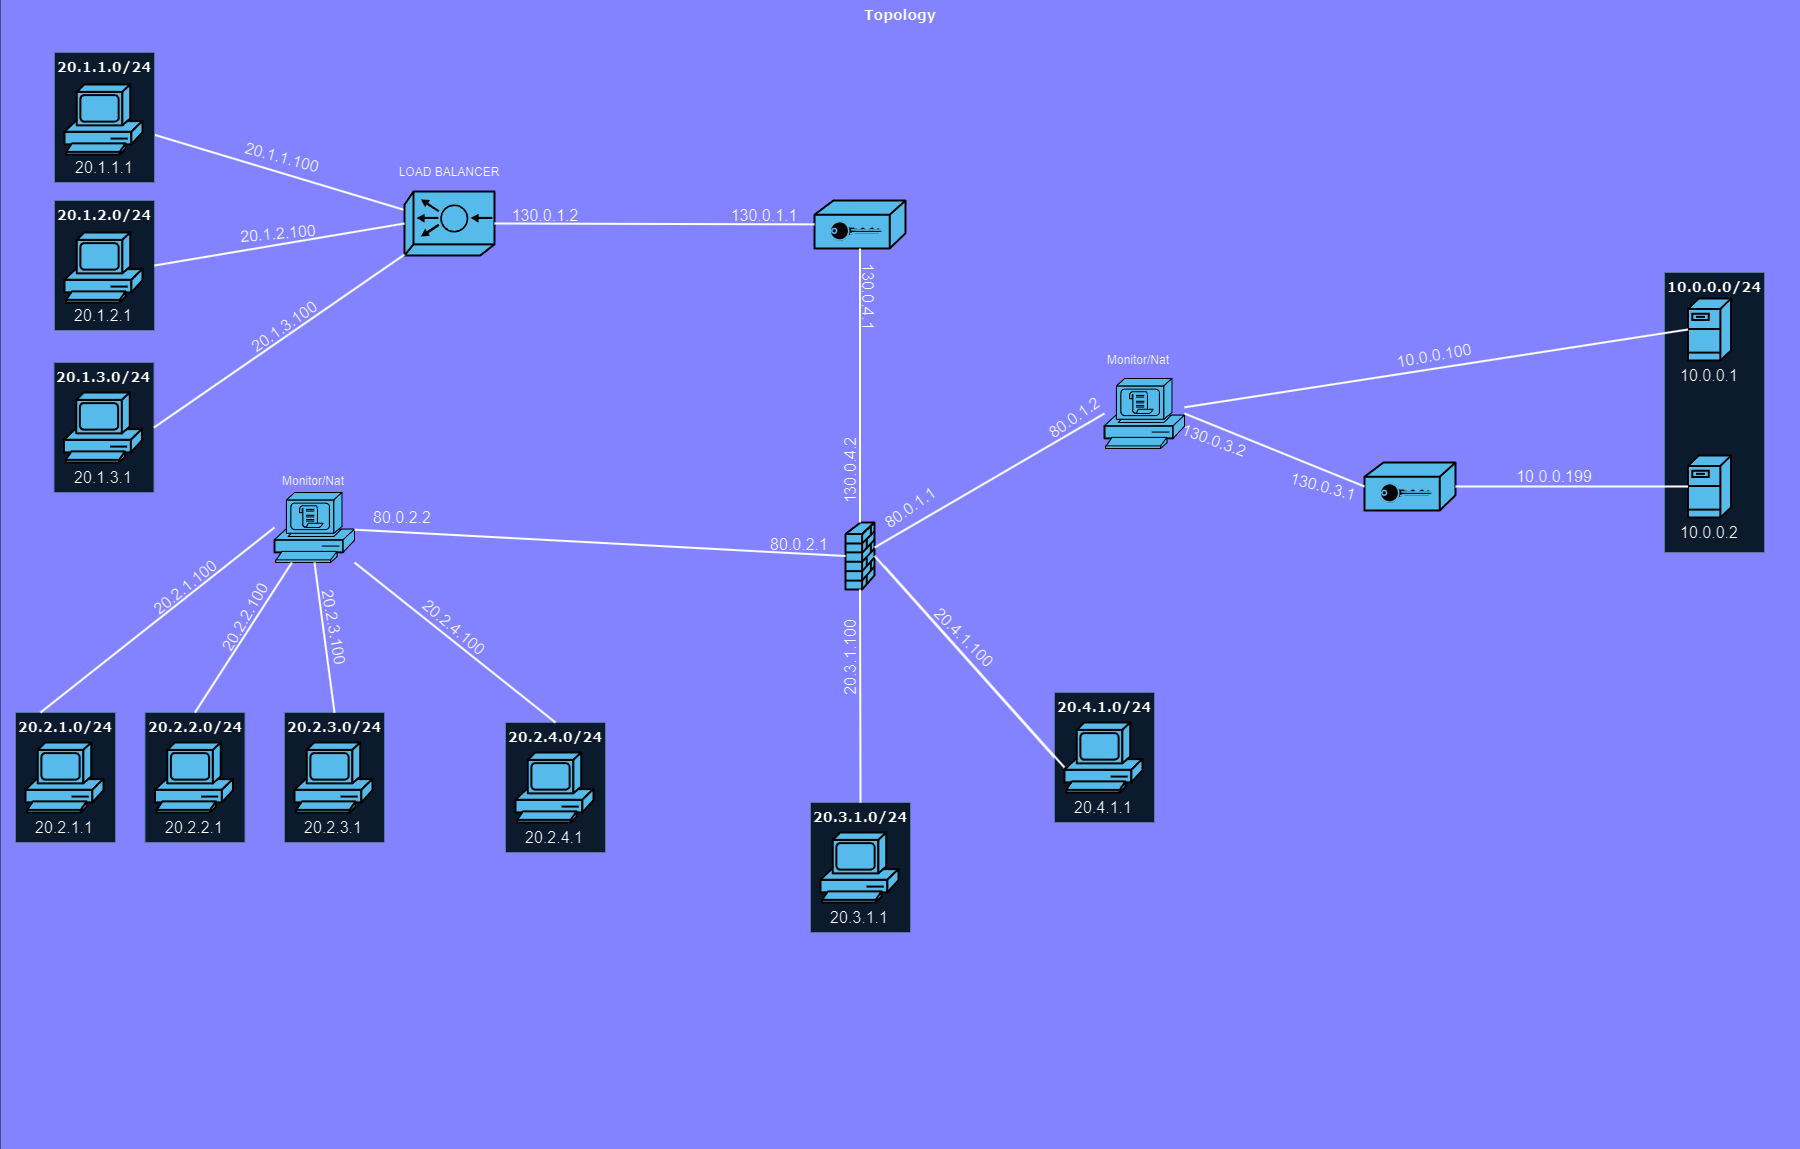
\includegraphics[width=1\textwidth]{Topologia_finale.png} 
    \caption{Verefoo Output}
    \label{fig:VPNDeploy}
\end{figure}

Come ci si poteva aspettare, dati i requisiti di sicurezza definiti sono state allocate tre Network Security Functions. Al centro della topologia è stato inserito un Firewall, che a prima vista sembra essere posizionato correttamente perchè in quella posizione riesce a scartare il traffico proveniente sia dalla
rete 20.1.*.*/16 che quello dalla rete 20.2.*.*/16. Ai lati sinistro e destro sono invece presenti i due VPN Gateway, occorre portare particolare attenzione a quello situato a sinistra in quanto il suo allocation places non era presente in input (figura \ref{fig:AllocationGraphB}), di conseguenza è possibile dedurre che dopo aver
istanziato una Network Security Function la successiva è stata posizionata in uno degli allocation places aggiuntivi formati nella nuova versione del framework.

\subsection{Configurazioni Network Security Functions}
Data la posizione che sembra definire una soluzione plausibilmente corretta, è possibile analizzare anche le configurazioni fornite per ogni funzione di sicurezza.
La seguente è la tabella che descrive la configurazione dei due gateway VPN:

\begin{table}[H]
    \centering
    \begin{tabular}{ccccccc}
        \hline
         Name & Action & IPSrc & IPDst & pSrc & pDst & tProto \\
        \hline
        VPN1 & ACCESS & 20.1.1.1 & 10.0.0.2 & * & 22 & ANY \\
        VPN2 & EXIT & 20.1.1.1 & 10.0.0.2 & * & 22 & ANY \\
        \hline
    \end{tabular}
    \caption{Configurazione dei due VPN gateway Demo B}
    \label{tab:tabella}
\end{table}

Come si può notare, dato l'unico requisito di protezione che era stato definito, solo due gateway sono stati allocati, rispettivamente di accesso per quanto riguarda il gateway presente a sinistra, e di uscita per quello di destra.
In entrambe le configurazioni si può notare che il singolo host dal quale comunicazioni dovranno essere cifrate è la sorgente 20.1.1.1, mentre il nodo di destinazione è il server S2 definito dall'IP 10.0.0.2. Anche i requisiti sul protocollo di trasporto
sono verificati in quanto la porta di destinazione che il server deve ricevere è la 22 che è quella indicata nei requisiti ed inoltre anche nella configurazione non c'è nessun vincolo di protocollo tra TCP e UDP.\\
Per quanto riguarda invece la configurazione del firewall, Verefoo fornisce il seguente output:

\begin{table}[H]
    \centering
    \begin{tabular}{ccccccc}
        \hline
        Default Action & Action & IPSrc & IPDst & pSrc & pDst & tProto \\
        \hline
        ALLOW & DENY & 20.1.*.* & 10.0.0.1 & * & * & ANY \\
        ALLOW & DENY & 20.2.*.* & 10.0.0.2 & * & * & ANY  \\
        \hline
    \end{tabular}
    \caption{Configurazione Firewall Demo B}
    \label{tab:tabella}
\end{table}

Anche in questo caso il framework sembra produrre una soluzione plausibile, in quanto il Firewall è stato configurato in blacklist, permettendo a qualsiasi traffico il transito tranne a quello 
definito nelle regole specifiche del firewall. In questo modo è possibile far comunicare tranquillamente le sottoreti 20.3.1.0/24 e 20.4.1.0/24 in quanto qualsiasi pacchetto da e per i due server S1 ed S2 non verrà
mai scartato dal firewall. Viceversa per quanto riguarda le sottoreti 20.1.0.0/16 e 20.2.0.0/16 il framework non solo ha prodotto delle regole corrette, ma è riuscito anche a raggruppare tutte le definizioni singole sulle reti più piccole in una
definizione più generale grazie alla notazione con \textit{"*"}. Tramite ciò quindi ogni elemento appartenente alla sottorete 20.1.0.0/16 non potrà comunicare con il server S1 ed ogni elemento nella rete 20.2.0.0/16 non potrà comunicare con il server S2.

\subsection{Configurazioni Strongswan}
Nonostante le configurazioni della topologia e delle network security function siano corrette, il framework prodotto allo stato attuale non fornisce una implementazione aggiornata del Translator di Strongswan, non è quindi possibile ottenere automaticamente 
una versione aggiornata dei file di configurazione "swanctl.conf". Per aggirare questo problema, durante lo sviluppo di questa Demo i file di configurazione dei due Gateway sono stati prodotti manualmente a partire dalle configurazioni fornite da Verefoo. \\
Di conseguenza, il seguente snippet di codice rappresenta uno dei due file di configurazione scritti per testare l'ambiente virtuale:

\begin{lstlisting}[language=sh]
    connections {
   site-site {
      local_addrs  = 130.0.4.1
      remote_addrs = 130.0.3.1
      local {
         auth = pubkey
         certs = VpnConfig1Cert.pem
         id = VpnConfig1.strongswan.org
      }
      remote {
         auth = pubkey
         id = VpnConfig2.strongswan.org
      }
      children {
         net-net {
            local_ts = 20.1.1.1/32            
            remote_ts = 10.0.0.2/32            
            start_action = trap|start 
            rekey_time = 5400
            rekey_bytes = 500000000
            rekey_packets = 1000000
            esp_proposals = aes256-sha2_256-modp2048
         }
      }
      version = 2
      mobike = no
      reauth_time = 10800
   }
   
}
\end{lstlisting}

All'interno di questo esempio la connessione site-to-site è definita dalle interfacce dei due VPN gateway con IP 130.0.4.1 e 130.0.3.1. In locale vengono caricati i certificati attraverso
il file VpnConfig1Cert.pem e l'autenticazione viene effettuata tramite chiave pubblica asimmetrica, in maniera simile viene definito l'id e il metodo di autenticazione del gateway remoto.
Infine viene dichiarata una connessione end-to-end tra il client C1-1 definito da 20.1.1.1/32 e il Web Server S2 definito da 10.0.0.2/32. All'interno di questa connessione viene definita anche la proposta
da effettuare per l'incapsulamento in IPSec tramite il protocollo ESP, utilizzando gli algoritmi di aes256-cbc e sha2-256.

\section{Verifiche e Test}

Grazie alle configurazioni prodotte in output dalla nuova versione del framework è possibile verificare che le soluzioni prodotte siano efficaci e corrette.
Per fare ciò, come nella demo precedente è stato predisposto un ambiente virtuale composto da container Docker che simuleranno il comportamento di ogni elemento di rete descritto nella topologia. In questo caso
le verifiche da effettuare all'interno della topologia saranno diverse perchè non sarà necessario dimostrare solo che le comunicazioni fra l'host C1-1 ed il server S2 siano protette tramite crittografia ma è anche
necessario controllare se le comunicazioni fra i client ed i vari host vengono filtrate dal firewall. \\
Partendo dalla verifica del firewall sarà necessario utilizzare due terminali differenti, il primo corrispondente al client C1-1 che come da requisiti dovrebbe essere in grado di comunicare solo con il server S2, isolando tutte le
comunicazioni con S1. Per testare ciò utilizzeremo i seguenti comandi Linux:

\begin{figure}[H] 
    \centering
    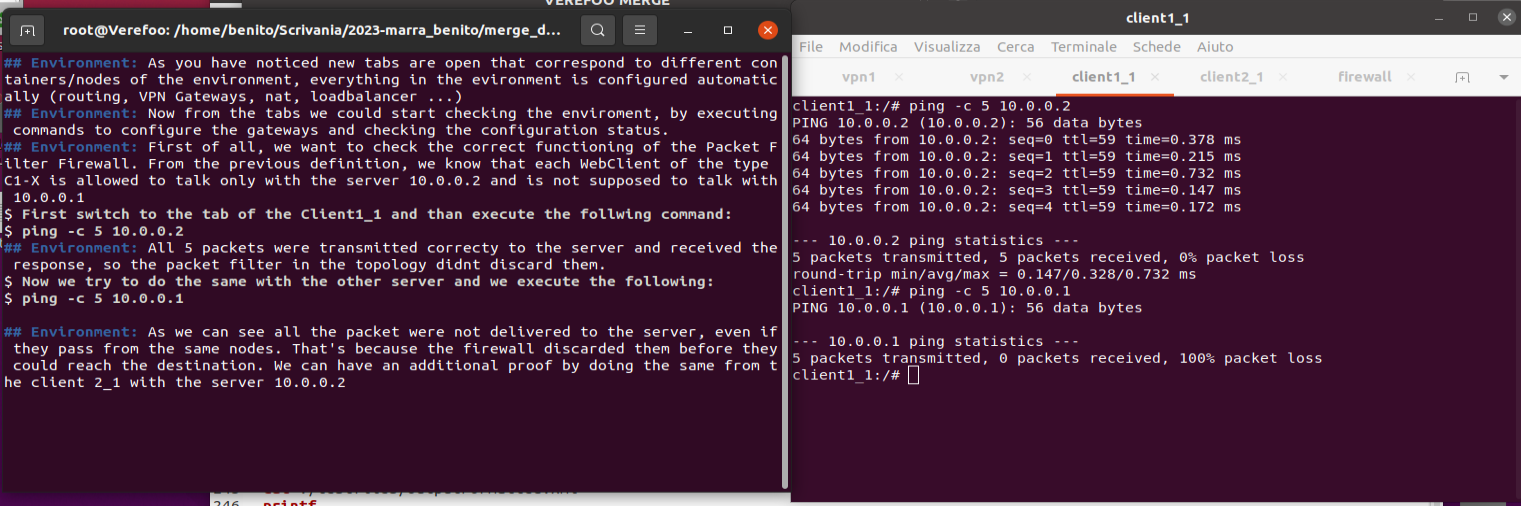
\includegraphics[width=1\textwidth]{(1)FirewallDiscard1.png} 
    \caption{Verifica pacchetti scartati dal Firewall per rete 20.1.*.*}
    \label{fig:Verifica1}
\end{figure}

All'interno del terminale C1-1 eseguiamo il comando \textit{"ping -c 5 [ipaddr]"} per verificare le connessioni con i due server presi in esame.
Nel primo caso testiamo sul server dall'IP "10.0.0.2" ovvero S2: come si può notare vengono trasferiti 5 pacchetti col protocollo ICMP e contemporaneamente vengono
ricevuti 5 pacchetti con una statistica di 0\% packet loss. Se invece eseguiamo la stessa operazione con il server dall'IP "10.0.0.1" il risultato sarà opposto, ovvero tutti
i pacchetti inviati vengono scartati non ricevendo alcuna risposta ed il numero di packet loss sarà uguale al 100\%.\\
Considerando il percorso che eseguono i pacchetti, ovvero\\
 $ \text{C1-1} \rightarrow \text{Lb} \rightarrow \text{VPNGateway1} \rightarrow \text{Firewall} \rightarrow \text{Monitor} \rightarrow \text{VPNGateway2} \rightarrow \text{Server}$
è possibile dedurre che l'elemento che scarta i pacchetti e impedisce le comunicazioni è proprio il firewall con la configurazione prodotta da Verefoo.\\
Tuttavia verificare le comunicazioni fra il client C1-1 ed il Server S2 non è sufficiente a verificare il corretto funzionamento del firewall, è infatti necessario assicurarsi che anche
le comunicazioni all'interno della rete 20.2.0.0/16 vengano filtrate quando si prova a comunicare con il server S1. 
\begin{figure}[H] 
    \centering
    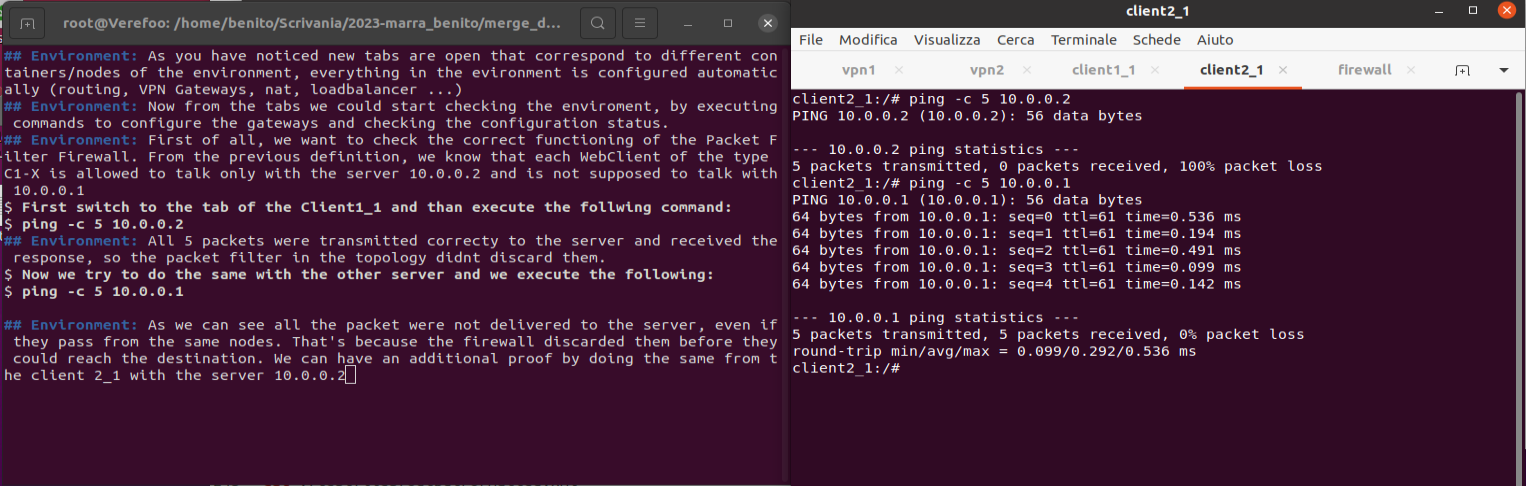
\includegraphics[width=1\textwidth]{(2)FirewallDiscard2.png} 
    \caption{Verifica pacchetti scartati dal Firewall per rete 20.2.*.*}
    \label{fig:Verifica2}
\end{figure}

Per verificare anche questa condizione vengono effettuati gli stessi comandi sul terminale del client C2-1, avendo un IP appartenente alla rete 20.2.0.0/16.
Il risultato che viene visualizzato in output è coerente con quello che ci si aspetta, essendo opposto all'output del client C1-1. Le comunicazioni con il server
10.0.0.2 non risultano possibili in quanto ogni pacchetto è stato scartato dal Firewall ed è presente anche qua il 100\% di packet loss, viceversa quando si fa un ping 
sul server 10.0.0.1 corrispondente a S1 ogni pacchetto viene correttamente trasmesso e ricevuto dal server, passando quindi i controlli del firewall. \\
È quindi possibile affermare che le configurazioni riguardanti i requisiti di raggiungibilità e di isolamento prodotte dal framework risultano corrette e con il minimo uso 
di risorse possibili, in quanto grazie ad un unico firewall sono state soddisfatte tutte le caratteristiche fornite in input. \\ \\
La successiva verifica che deve essere effettuata sulla bontà della soluzione prodotta riguarda l'istanziazione e la configurazione dei VPN Gateway nella topologia di output.
In questa istanza specifica solo 2 gateway sono stati allocati, quindi è sufficiente verificare che i pacchetti in transito tra il nodo C1-1 ed il server S2 risultano cifrati
correttamente. Prendendo spunto dai test effettuati nella demo precedente utilizziamo tcpdump nel seguente modo:

\begin{figure}[H] 
    \centering
    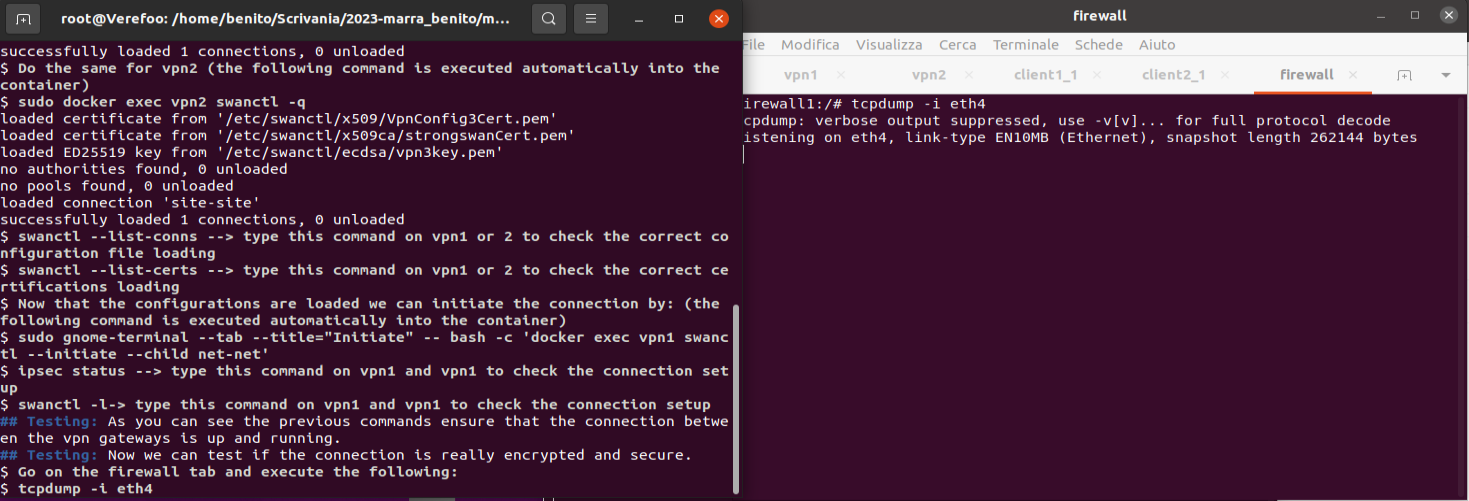
\includegraphics[width=1\textwidth]{(3)Firewall_tcpdump_setup.png} 
    \caption{Setup tcpdump per verifiche di sicurezza}
    \label{fig:Verifica3}
\end{figure}

Il nodo preso in analisi è lo stesso in cui viene instanziato il firewall, utilizzando tcpdump è possibile  osservare e monitorare i pacchetti in transito attraverso una delle interfacce
del nodo. L'interfaccia scelta per questo test è "eth4" corrispondente alla connessione fra il firewall ed il primo VPN Gateway. Il risultato aspettato è quindi, come per la prima demo, osservare
il transito dei pacchetti non come semplici ICMP packets ma come ESP packets, ovvero il protocollo utilizzato per l'incapsulamento in IPsec.\\
Per controllare l'output è quindi necessario, una volta impostato il monitoraggio dell'interfaccia, eseguire il comando di ping come fatto per il firewall precedentemente e controllare l'output 
nel terminale del firewall. Di seguito viene proposto un possibile output effettuato: 


\begin{figure}[H] 
    \centering
    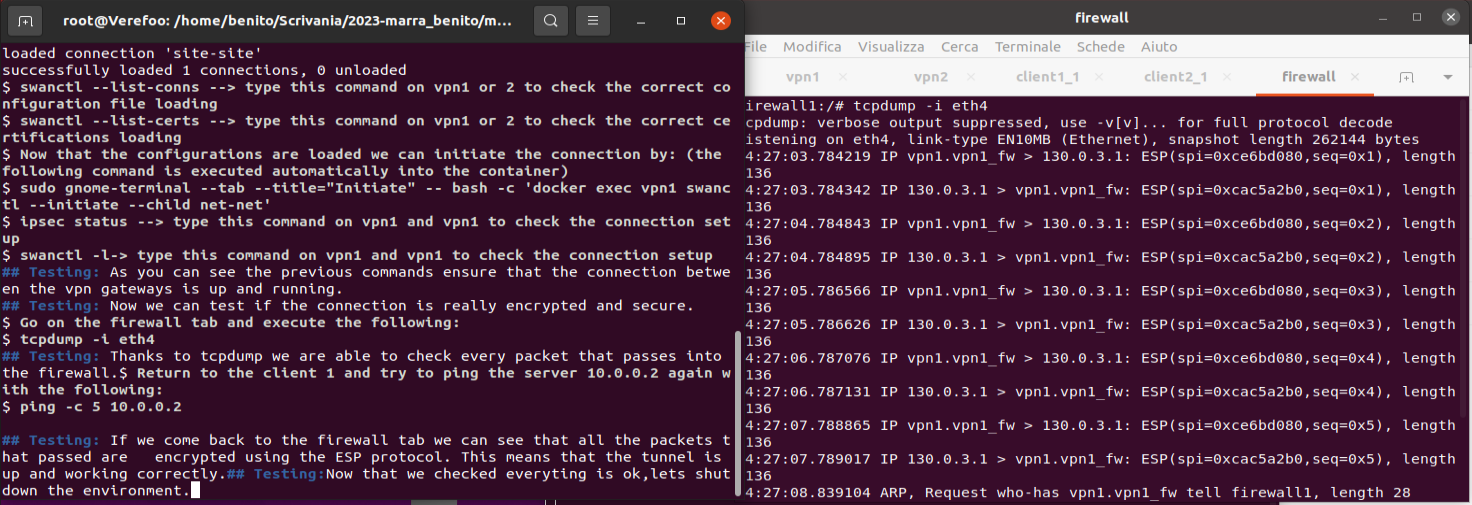
\includegraphics[width=1\textwidth]{(4)Encryptedpacket_output.png} 
    \caption{Verifica cifratura dei pacchetti in transito}
    \label{fig:Verifica4}
\end{figure}

Il risultato ottenuto corrisponde alle aspettative descritte precedentemente. È infatti possibile notare come ogni pacchetto venga codificato con il protocollo ESP e venga monitorato con il path specifico del tunnel VPN.
Di conseguenza è possibile affermare che il risultato prodotto da Verefoo è corretto in quanto garantisce la sicurezza in tutto il traffico partente dal nodo C1-1 al server S2. Grazie a questa ennesima verifica anche i requisiti
di sicurezza sono rispettati, confermando la correttezza del framework e della demo prodotta. Di conseguenza si può affermare che anche il terzo ed ultimo obiettivo della tesi è stato portato a termine, producendo una demo funzionante che
mettesse in risalto le caratteristiche della nuova versione del framework.


\chapter{Conclusions} \label{ch:conclusions}

Conclusion and future works
\bibliographystyle{IEEEtran}
\bibliography{bibliography}
%\include{bibliography}

%if appendixes are needed, uncomment the following lines
%\appendix
%\appendixpage
%\include{appendixA}
%\include{appendixB}



\end{document}

